%
%  愛知工業大学経営情報科学部情報科学科
%    コンピュータシステム専攻用LaTeXテンプレート(2015.12.22)
%
\documentclass[openany]{jbook}

% 使いたい人は使う
\usepackage{personal}

% 図挿入用
\usepackage[dvipdfmx]{graphicx}
\usepackage{latexsym}
\usepackage{amsmath,amssymb}
\usepackage{amsfonts}
\usepackage{ulinej}
\usepackage{url}
\usepackage{mathtools}
\usepackage{here} % 強制的に図を好きな位置に配置するためのパッケージ
\usepackage{multirow}
\usepackage{otf}



%化学記号用
% \usepackage[version=3]{mhchem}

% 丸付き数字の表示用
\newcommand{\marub}[1]{\raise0.2ex\hbox{\textcircled{\scriptsize{#1}}}}
\def\maru#1{\leavevmode\setbox0\hbox{$\bigcirc$}\copy0\kern-\wd0 \hbox to\wd0{\hfil{\scriptsize#1}\hfil}}

\pagestyle{headings}

% カウンタセット
\setcounter{secnumdepth}{3}
\setcounter{tocdepth}{3}

% 定義環境
\newtheorem{definition}{定義}[section]

% 例環境
\newtheorem{example}{例}[section]

% 新しい環境の定義
\newenvironment{indention}[1]{\par
\addtolength{\leftskip}{#1}
\begingroup}{\endgroup\par}

% 関連図書→参考文献
\renewcommand{\bibname}{参考文献}

\topmargin=-14mm
\headsep=15mm
\textwidth=15.7cm
%\baselineskip=22pt
%\renewcommand{\baselinestretch}{1.4}
\textheight=24.5cm  % 33 lines in 1 page
\oddsidemargin=7.5mm
\evensidemargin=7.5mm

% 部分コンパイル用
%\includeonly{title,chap1,chap2,chap3,chap4,chap5,thanks,reference}
\begin{document}

\begin{titlepage}

\ \\
\begin{center}

{\LARGE 愛知工業大学情報科学部情報科学科\\
コンピュータシステム専攻

\vspace{1.0cm}

令和2年度~卒業論文\\

\vspace{2.0cm}
{\Huge 
\baselineskip=15mm
\textbf{物体に設置したBLEビーコンの\\受信電波強度を用いた状態推定と\\その応用に関する研究\\}}

\vspace{7.0cm}

2021年2月\\

\vspace{1.0cm}

\begin{tabular}[h]{lll}
  研究者  & K17028 & 大鐘勇輝\\
         & K17124 & 水野涼雅\\
\end{tabular}

\vspace{1.0cm}

指導教員\ \ 梶 克彦\ \ 准教授}

\end{center}

\end{titlepage}
%%% Local Variables: 
%%% mode: latex
%%% TeX-master: "root"
%%% End: 
    

%目次を自動的に作る。
\tableofcontents

% 本文
\chapter{はじめに}
\thispagestyle{myheadings}

% **DIOCOMO2019 ========================================================**
\section{背景および研究目的}

通信インフラの整備とIoTの発展により,現在では様々なモノがインターネットに繋がるようになった.
エアコンや照明,家の鍵から車に至るまで,数年前ではインターネットとは無関係だったものが今では当たり前のようにインターネットに接続されている.
IoTに対応した家電は遠隔からの操作や機器の状態の通知,使用ログの保存が可能であり,例えばIoTに対応したエアコンでは家の外から電源のON・OFFや電気使用量のログの確認ができる.
そうした利便性から日々新たなIoT家電が生み出され続けており,総務省が公開している資料\cite{soumusyo}によると2020年には約300億のIoTデバイスが稼働していると予想されている.
IoTデバイスの増加により家中にそれらが設置されると,そこから得られる使用データから行動パターンといったライフログのデータが取得できる.
ライフログのデータは,環境に合わせた電力制御や老人の異常行動の検知など幅広い分野への応用が期待できる.


\section{hogehoge}

\section{huga}
\subsection{hugahuga}
\subsubsection{hugahugahuga}


\begin{equation}
  \begin{split}
      &\mbox{活動量(kcal)} \\
      &= \mbox{METs} \times \mbox{体重(kg)} \times \mbox{時間(h)} \times 1.05 \label{CalFormula}
  \end{split}
\end{equation}

% \labelの後の文字列は参照の際に使う

しかし,これらのデータはIoTに対応した家電でないと取得できず,金庫や椅子,扉といった家電以外のモノではセンサが無いためデータ収集が不可能という問題がある.
この解決策として,(1)加速度センサや回転センサといったモーションセンサを使う方法や,(2)Wi-Fi電波のチャネル状態情報を用いる方法がある.
(1)の方法は直接モノの動きを観測できるため安定した精度で状態推定ができる反面,センサ単体での動作が難しく取得したデータの保存・解析に専用の機器が必要である.
また,(2)の方法では対象物のそれぞれにセンサを付ける必要が無い一方,状態の推定にWi-Fi電波の反射波を用いるという特徴から小さな対象物への適用は不向きである.

そこで,本研究では汎用的な機器のみで動作でき,かつ小さな対象物でも高い精度で状態推定できる手法を提案する.
具体的には日常の生活空間内における家電・家具の内部にBluetooth Low Energyビーコン(以降,BLEビーコンと呼称)を設置し,送信される電波をスマートフォンで受信した際の受信電波強度をもとにモノの状態推定を行う.
これまでBLEビーコンは広告配信や位置推定のための電波を発する文字通り「ビーコン」として使用されてきたが,物体内部に設置し「センサ」としての使い方をされている例はあまりない.
BLEビーコンから発信される電波は微弱であるため,障害物の有無により電波強度が変化しやすい.
そのため,モノの状態変化に合わせて受信電波強度にも変化が現れやすく,状態推定に適している.
また,モノにおける状態推定を行うとき,電池交換といった管理コストや機器の導入コストは少ない方が望ましい.
その点,BLEビーコンは省電力なため長期間の稼働が可能であり,サイズ・重さともに小さいため設置も容易である.
加えてBLEビーコンの電波はスマートフォンで受信できるため,電波の受信に特別な機器を必要とせず,UUID,major,minorの情報から各BLEビーコンの識別ができるため,1台のスマートフォンで複数のBLEビーコンの監視が可能である.

ただし,BLEビーコンの電波は微弱であるがゆえ,モノの状態変化に関係ないノイズの影響を受けてしまい,正常に推定を行えない可能性がある.
また,推定対象物の材質によっては状態が変化しても受信電波強度にあまり変化がでない場合も考えられる.
これら問題を解決するため,本研究では測定した電波強度情報へのデジタル処理とハードウェアの設置に工夫を行い,安定した状態推定を実現する手法を提案する.




% **DIOCOMO2020 (ryoga)====================================================**
\section{BLEビーコンを用いた状態推定の高齢者モニタリングへの応用}
\label{sec:example}

本研究では最終目標として,BLEビーコンを用いた状態推定の高齢者モニタリングへの応用も目指す.
日本では医療技術の発達や公衆衛生活動の発展より人の寿命が年々伸び続けており,厚生労働省が公開している『平成30年簡易生命表』\cite{AveLife}によると,2018年時点の平均寿命は男性が約81年,女性が約87年と公表されている.
この数字は1947年の平均寿命が男性は約50年,女性は約54年だという事実から考えると,71年間で男女ともに30年以上伸びている.


この平均寿命の延伸に伴う高齢化によって,要介護人や寝たきり状態の人も増加しており,ベッドや布団上での行動把握が介護人にとって重要になりつつある.
なぜならベッドや布団上での行動が把握できると,それを健康管理に繋げられるからである.
例えば,人は眠りの深さにより移動量が異なるため,寝返り回数などが把握できるとそこから睡眠の質を推定できる.
また要介護者がベッドや布団上で過ごす際,長時間同じ姿勢で寝ていると褥瘡発症の可能性が高まる.
同じ姿勢で寝ていると,一定の箇所に圧力がかかってしまうため血流の悪化や,汗や尿等による汚れにも繋がる.
そのため,介護人による定期的な体位の変更やシーツや衣服の取替,スキンケアなどが必要になる\cite{jokusou, mekanizumu}.
褥瘡を発症させないためには予防が重要となり,ベッド上での行動や睡眠位置の把握は様々なケアの指標になりうる.
褥瘡は介護を行う上で深刻な問題となっている.

褥瘡とは皮膚や皮膚の下部組織の損傷であり,長時間同じ姿勢で過ごし一定の箇所への圧力が継続した場合に発症する.
長期に渡り圧力がかかると血流が悪くなり,その結果皮膚組織に酸素や栄養が行き渡らなくなってしまい損傷してしまう.
一般的に褥瘡の重症度は6つのレベルに分類\cite{level}されており,軽い場合には皮膚が赤くなる程度だが,重症になると最終的には傷が筋肉や腱,骨にまで到達してしまう.
褥瘡の治療には除圧や最悪の場合手術が必要になり当人や介護人の負担が大きくなってしまうため,予防が重要となる.
そこで,1つ目の応用例としてBLEビーコンを用いた睡眠位置認識を提案する.

% **DIOCOMO2020 (ogane)====================================================**
また,平均寿命の延伸によって近年では人生100年時代と呼ばれるようになり,WHO(世界保健機関)はこれからは単に寿命を延ばすのではなく,健康寿命を延ばしていくのが大切だと提唱している.
健康寿命とはWHOが「健康上の問題で日常生活が制限されることなく生活できる期間」\cite{WHO}と定義したもので,この延長が実現できれば介護人の負担を軽減できるほか,医療費の削減に繋げられるだろうと期待されている.
健康寿命を延ばす重要な要素として,適度な運動やバランスの良い食事,質の高い睡眠などが挙げられるが特に運動に注目して考えてみると,運動量を知る指標として歩数を確認する方法が挙げられる.
歩数は単純に足を動かした回数であるため運動量の目標が立てやすく,その算出も容易である.

しかし,歩数は自立して歩ける人のみに適用できる指標であり,車椅子使用者ではこの指標を用いた運動量の推定は不可能である.
これまで車椅子における移動認識の先行研究として,GPSを用いた手法\cite{gps}や加速度,角速度,地磁気を用いた手法\cite{baske}など様々な手法が提案されてきた.
\cite{gps}の手法はGPS電波が受信できる屋外では高精度な位置推定が実現できる反面,GPS電波が届かない屋内では利用できないという問題がある.
また,\cite{baske}の手法はセンサを取り付けて直接車椅子の動きをセンシングするため,屋外・屋内のどちらでも位置推定ができる一方,定期的に電池交換といったメンテナンスが必要である.
本応用例は介護施設や老人ホームといった施設で,職員が車椅子を使用する入居者の健康管理を行うシーンを想定している.
そのため,低コストで導入でき,かつ電子機器の取り扱いに慣れていない人でも運用を行えるのが望ましい.
そこで,2つ目の応用例としてBLEビーコンを用いた車椅子の移動認識手法を提案する.

\section{論文構成}
本稿の構成は以下の通りである.
2章では,屋内日常物における状態推定に関する既存研究を紹介し,その問題点を述べる.
3章では,BLEビーコンを使用したモノの状態推定について述べ,その評価・考察を行う.
4章・5章では,BLEビーコンを用いた状態推定の応用例について述べる.
最後に6章で,本研究のまとめを行う.
\thispagestyle{myheadings}
\chapter{関連研究}

% DICOMO2019 ########################################################################################################
\section{モノの状態推定に関する関連研究}
室内にあるモノの状態推定には,加速度センサや振動センサなどを利用する方法やWi-Fiの電波を利用する方法など様々な手法が提案されてきた.
前川ら\cite{TagAndThink}は様々なセンサを搭載したセンサノードをモノに取り付け,そこから得られるセンサ情報と事前に用意しておいたそのモノ固有の状態遷移図を比較し,自動でモノの状態と何に付けられているのかを推定している.
角速度や照度などから,センサノードが取り付けられている状況や状態変化を検出するという手法である.
この手法ではセンサノードがどんなモノに付いていて,どんな状態変化をしたか推定が可能である.

消費電力の変化から電気機器の状態推定を行っている研究がいくつかある.
例えば,機器やコンセントごとの消費電力を計測できる細粒度電力センサを使用し,電気機器の電力消費の変化から浪費電力の検出・分類が行われている\cite{sairyu}.
その他にも電気機器の運転モードの切り替えや開閉などの状態変化によって起こる消費電力の変化から状態の推定を行い,そこから得られる時系列の情報から人物の位置推定が行われている\cite{energy}.
これら二つの手法では,電気機器の状態変化から起こる消費電力の増減に着目し推定を行っているため,電化製品に対しては有効な手法ある.
一方で,電気を用いない家具や雑貨に対しては適用が不可能である.

Wi-Fi電波を用いて,室内状況や人の状態を推定する研究がある.
例えば室内状況の推定では,Wi-Fiのチャンネル状態情報を用いてドアの開閉検知\cite{WifiChannel}や通過検知\cite{LANgate},会議室の状態検出\cite{Room-State}が行われている.
また,人の状態推定では呼吸の検出\cite{Human-Respiration}や失神検知\cite{WiFi-Toilet}が行われている.
これらの研究は,Wi-Fi電波を利用するという理由から推定対象物にセンサを取り付ける必要が無く,導入が簡単に行える.
しかし,電波の状態を推定の指標とするため,小さいモノや頻繁に移動を伴うモノでは状態変化の推定が難しい.

そこで,これらの問題の解決策として本研究ではBLEビーコンを用いる.
BLEビーコンは,低消費電力であるため長期間の稼働が可能であり,電池交換といった運用コストを小さくできる.
また,小型・軽量という特徴から設置が容易で,直接モノの内部への設置も可能である.
このような特徴から,マーケティング\cite{bleUse}から在室検知・位置推定まで幅広く活用されている.
在室検知では,BLEビーコン電波のRSSI値を用いて在室を推定する研究が行われている\cite{home-location, stay-estimation, en-AreaUsed, Finding_by_Counting, dakoku_system, makoto, konzatsu}.
また,距離や障害物の有無によって変化する電波強度をもとに,位置や状態を推定する研究が数多く行われている\cite{move-tracking, BLE-Localization, IoMT, tandem, blespot, en-door}.
本研究では,これらの研究で利用されているBLEビーコンの特徴に着目し,日常の生活空間内におけるモノの状態変化の推定を行う.


% DICOMO2020(ryoga) ########################################################################################################
\section{睡眠位置認識に関する関連研究}
睡眠位置認識に関する研究は様々行われている.
ベッドの脚それぞれに荷重センサを取り付け位置を認識する研究\cite{ML}やサービスがあり,高齢化による需要の増加や介護業界の人手不足,介護人の負担増加といった問題を解決するために支援を行っている.
例えばリコーの見守りベッドセンサシステム\cite{riko}では,リアルタイムにベッド上での位置把握が可能であり,そこから活動量や離床のタイミングがわかる.
さらにそれらの情報は,ネットワークを介してナースステーションや家族の自宅から確認ができる.
しかし,導入には費用や手間がかかってしまうため在宅介護などで利用するにはハードルが高い.
またこの手法ではベッドの脚にセンサを取り付ける必要があるため,布団では適用が難しい.


布団にも適用できる睡眠位置認識では,圧力センサを用いた研究が多く行われている.
カメラを用いた動画像処理を行う研究\cite{Multimodal}もされているが,プライバシーや被撮影者負担などの観点から避けられる傾向にあり,代わりにセンサを用いた手法が多く提案されている.
西田らは221個の圧力センサを7cm間隔で並べた圧力分布測定シートを用いて,体位の測定に加え呼吸の測定を行っている\cite{atu}.
睡眠位置の判定には,圧力分布画像を処理し芯線を抽出する.
さらに芯線上の圧力最大地点の特徴から仰臥位と腹臥位を判別し,横隔膜の振幅の特徴と圧力分布を組み合わせて呼吸検出を行っている.


また近年ではシーツ型のセンサや,シーツや衣服といった布にセンサを織り込んだものが多く使用されている\cite{orimono, seat}.
岩瀬らは寝姿体圧画像から睡眠位置推定と関節位置推定を行っている\cite{kansetu}.
関節位置推定モデルに人物領域推定によるノイズ抑制と姿勢分類情報を組み込み推定を行う.% ←←←なんか変
また小野瀬らは衣類型のセンサを用いて圧力分布を計測しており,シーツ型センサとの比較を行っている\cite{irui_hikaku}.
これらの手法では,測定された圧力から特定の部位に負担がかかっていないか把握できるため,褥瘡対策に有効である.
しかし設置と使用には専用のセンサや装置が必要になるため,やはり一般の人では導入が難しい.





そこで我々は,BLEビーコンの受信電波強度を用いた睡眠位置認識手法を提案する.
BLEビーコンであれば家電量販店などで手軽に安価で入手でき,電波の受信もスマートフォンでできるため専用の装置を用意する必要が無い.
我々は以前,受信電波強度を用いた状態推定を提案しており,その手法をもとに位置認識を行う.


% DICOMO2020(ogane) ########################################################################################################
\section{車椅子の移動認識に関する関連研究}
車椅子の移動認識手法として,センサやGPS,カメラを用いた手法など様々な手法が提案されている.
%モーションセンサ
センサを用いた手法では,加速度センサや角速度センサ,ロータリエンコーダといった,モーションセンサを用いた手法が数多く提案されている\cite{en-Accelerometer, en-kalman}.
これらの手法は,車椅子に直接センサを取り付けてセンシングするため,正確な動きの情報が得られる.
しかし,この手法は測定データから得られる移動方向と距離をもとに,初期位置からの相対的な移動を推定していくものであるため,長距離移動した場合ズレが蓄積してしまう.
この問題に対処するため,長谷川らはBLEビーコンを用いて誤差を補正し,車椅子バスケにおける選手の位置推定を行う手法を提案している\cite{baske}.
車椅子に設置された受信機でBLEビーコンの電波を受信し,そのBLEビーコンIDと紐付けられた位置情報をもとに,位置誤差を修正するという手法である.
このようにモーションセンサを用いた手法では,位置誤差を修正する必要がある.

%GPS
位置誤差が蓄積しない手法として,GPSを用いた手法がある.
GPSは現在位置を緯度・経度の絶対座標として取得できるため,屋外において高精度な移動認識が実現できる.
この特徴を利用し,屋外の道路において左右どちらの歩道を通行したか推定する研究がある.
阿部らは,人のそばにある建物上空のGPS信号は受信し難いが,上が開けている車道側上空のGPS信号は受信されやすいという特徴に着目し,歩道単位での位置推定を実現している\cite{gps}.
この研究はGPS信号のみを使用して歩行通路判定を行うため,マップマッチングなどの補正をする必要がなく,実装が簡単に行えるメリットがある.
一方で,GPS信号は屋外でしか受信できないため,屋内での移動認識は不可能である.

%カメラ
屋内においても移動認識を実現する手法として,カメラを用いた手法がある.
この手法は,あらかじめ目印となる物とその座標を結びつけておき,カメラでその目印を検出して位置推定を行う.
この特徴を用いて車椅子ナビゲーション\cite{marker}や,軌道追跡\cite{en-baske}を実現する研究がある.
これらの研究は目印となる物を設置するだけで位置推定環境が整うため,専門知識がない人でも簡単に導入が行える.
しかしながら,目印の検出には画像処理が必要であり,計算量のコストが他の手法と比べて高いという問題がある.

%スマホセンサ
導入コストが低い移動認識手法として,スマートフォンに内蔵されたセンサを用いる手法がある.
ワッタナワラォンクンらは移動速度を測る車輪センサと,スマートフォンの方位センサを組み合わせて測位をしている\cite{navi}.
また,測位結果をもとに坂道や階段を回避した目的地への最適ルートを計算し,スマートフォン上に図面データと共に表示する.
この手法はスマートフォンをナビゲーションシステムとして使うだけでなく,測位のためのセンサとしても使用している.
そのため,モーションセンサだけを使用する手法と比べて導入コストを抑えられる.
岩崎らは室内の天井にスピーカを取り付け,そこから発せられる周波数の異なる音波をスマートフォンで受信し,測位する手法を提案している\cite{microphone}.
この手法は車椅子側にセンサを取り付ける必要が無いため,車椅子を多く使用する施設では導入コストの大幅な削減が実現できる.
一方で,スマートフォンは機種によってセンサ精度に違いがあるため,人によって得られる結果が異なる可能性がある.

%モーションセンサの応用例
通常,移動認識に使用される情報を他の用途に活用する研究がいくつか行われている.
まず,加速度センサの情報をもとに,車椅子使用者の消費カロリーを推定する研究がある.
谷本らは加速度の変化から車輪を漕いだ回数を推定し,その際の強度を3つのレベルに分類するという手法で車椅子使用時の消費カロリーを推定している\cite{en-calorie}.
この研究は加速度の情報から消費カロリーを算出しているため,移動認識と運動量推定が同時に実現できる.

また,センサデータに基づいたバリア情報の評価を目指す研究がある\cite{OperationModel, RoadEval, on-demand, en-Mahalanobis}.
通常,移動認識に使用される情報を活用して,歩道の傾斜や障害物といったバリア情報を発見・評価するという研究である.
これらの研究は,その評価したバリア情報から車椅子使用者の行動支援をできるだけでなく,障害物を目印として移動認識における位置誤差の修正にも応用が可能である.

\chapter{物体内部に配置したBLEビーコンの電波強度を用いた状態推定}
\thispagestyle{myheadings}

% 画像を書く時のやり方
% TBH トップボトムひあー
% 載せるとこるの場所を指定する
\begin{figure}[tbh]
    \centering
    % 画像のサイズを指定する
    % 画像の場所を相対パスで指定する。
    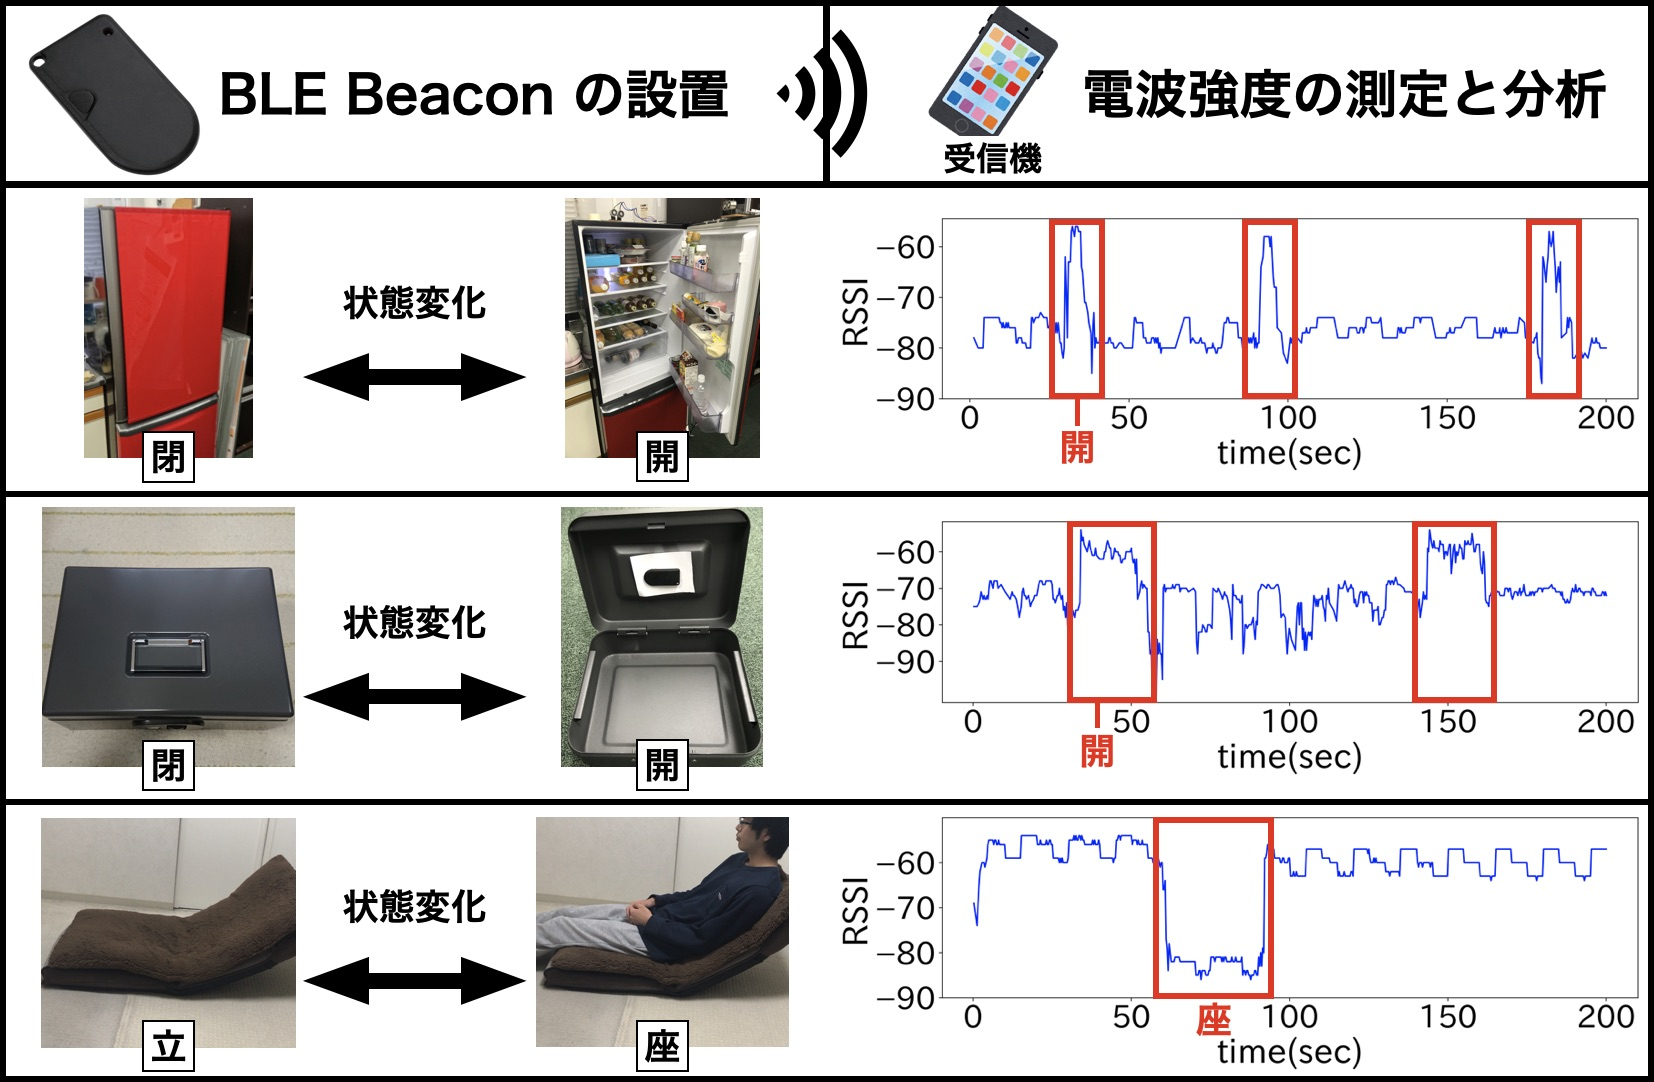
\includegraphics[width=14cm]{images/chapter3/abst.jpg}
    % 図の名前を決めれる。
    \caption{提案手法概要}
    % 図のラベルを決めれる。文章中からの参照を使える。
    \label{abst-chap3}
\end{figure}

本研究では屋内にあるモノの内部に直接BLEビーコンを設置し,その状態変化による電波強度の変化からモノの状態推定を行う.
% 画像の参照を指定する。「図1.1」を示すみたいなやつ
提案手法の概要図を図\ref{abst-chap3}に示す.
本稿では材質や使用方法によって受信電波強度に大きな変化が現れるモノを対象として,状態推定を行う.
具体的には,冷蔵庫と金庫,座椅子である.
冷蔵庫(図\ref{freezer})では扉の棚部分,金庫(図\ref{safe})では開閉する蓋の部分,座椅子(図\ref{chair})では人が座る座面の部分や背もたれの部分へ図\ref{beacon}のBLEビーコンを設置する.
冷蔵庫や金庫では金属による電波の減衰が起き,座椅子では人体によって電波の減衰が起こる.
これにより,扉の開閉や人の着座などのモノの状態変化からBLEビーコンの遮蔽状態が変化するため,外側に設置した受信機での受信電波強度が変化する.
この変化する電波強度をもとにモノの状態変化の推定を行う.


% 絶対表示させたいときはこっち『H』!!
\begin{figure}[H]
    \centering
    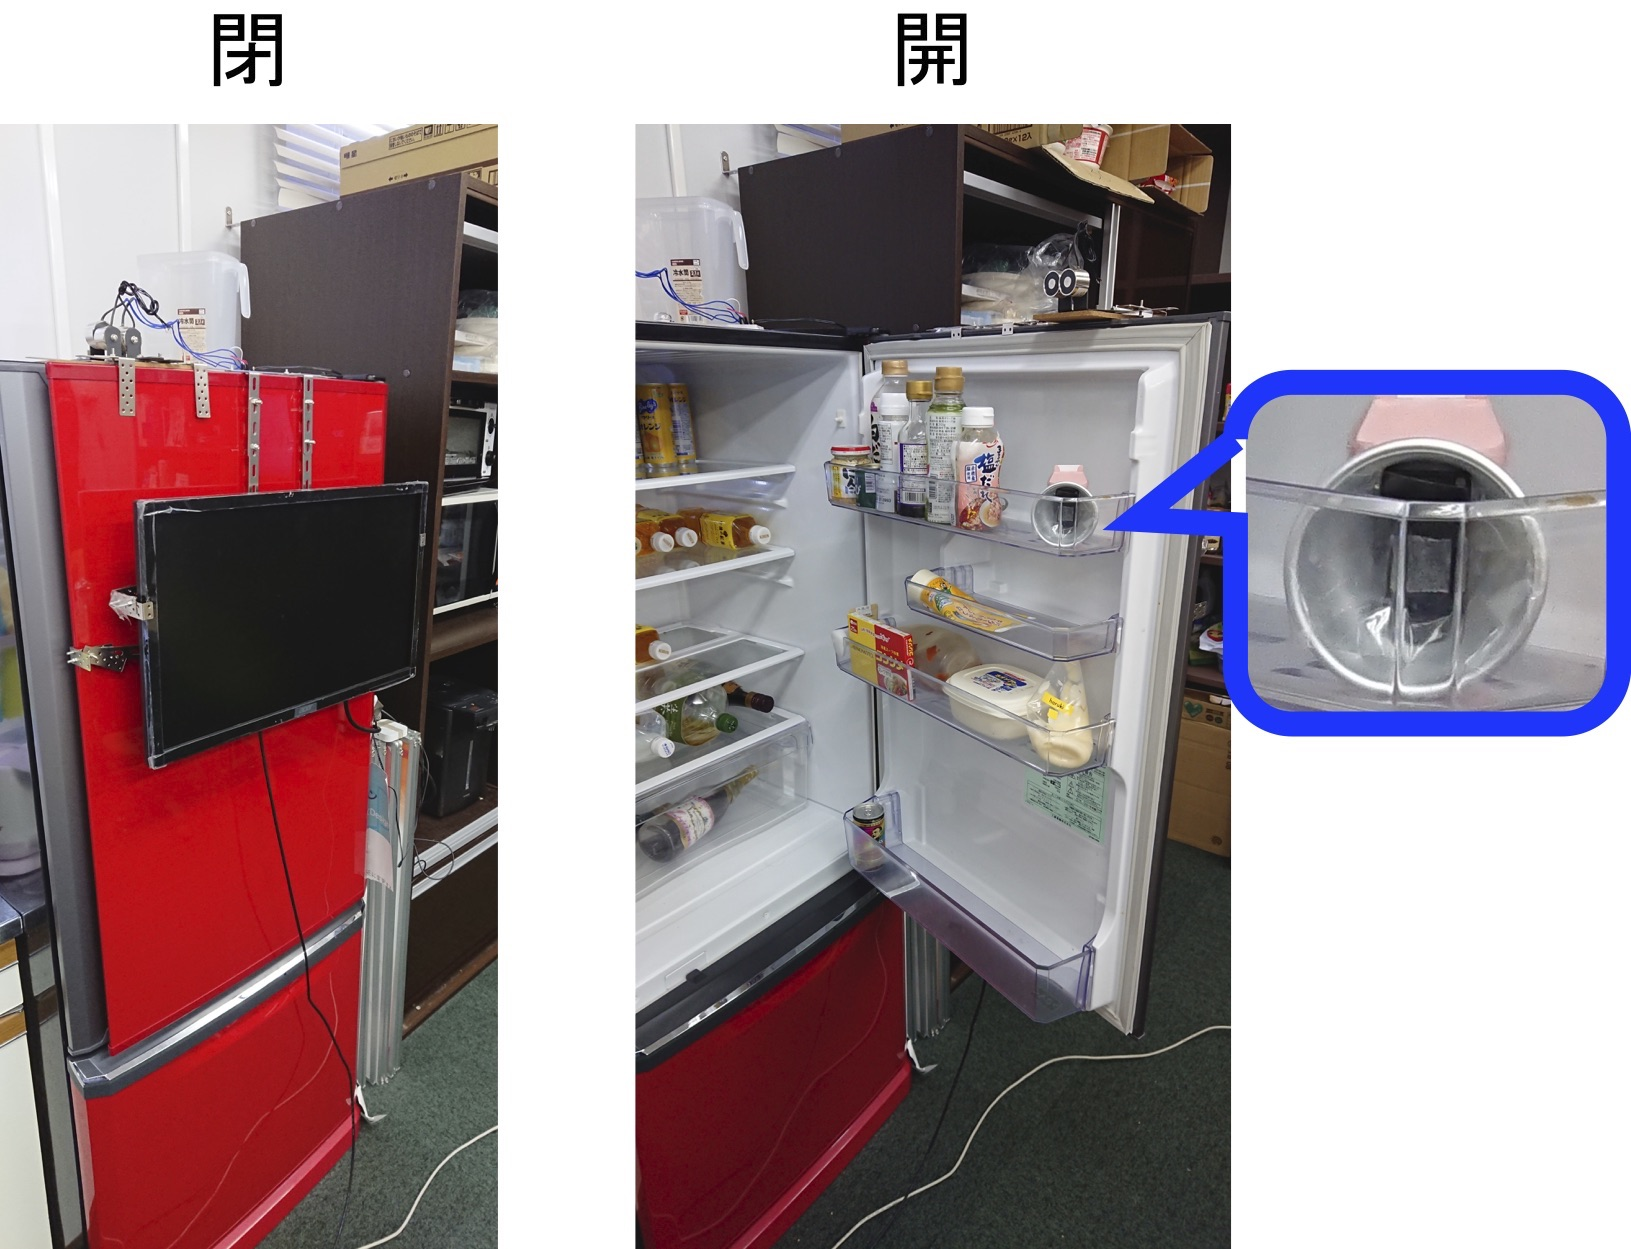
\includegraphics[width=10cm]{images/chapter3/regisW2.jpg}
    \caption{冷蔵庫の状態と設置したBLEビーコン}
    \label{freezer}
\end{figure}


\begin{figure}[H]
    \centering
    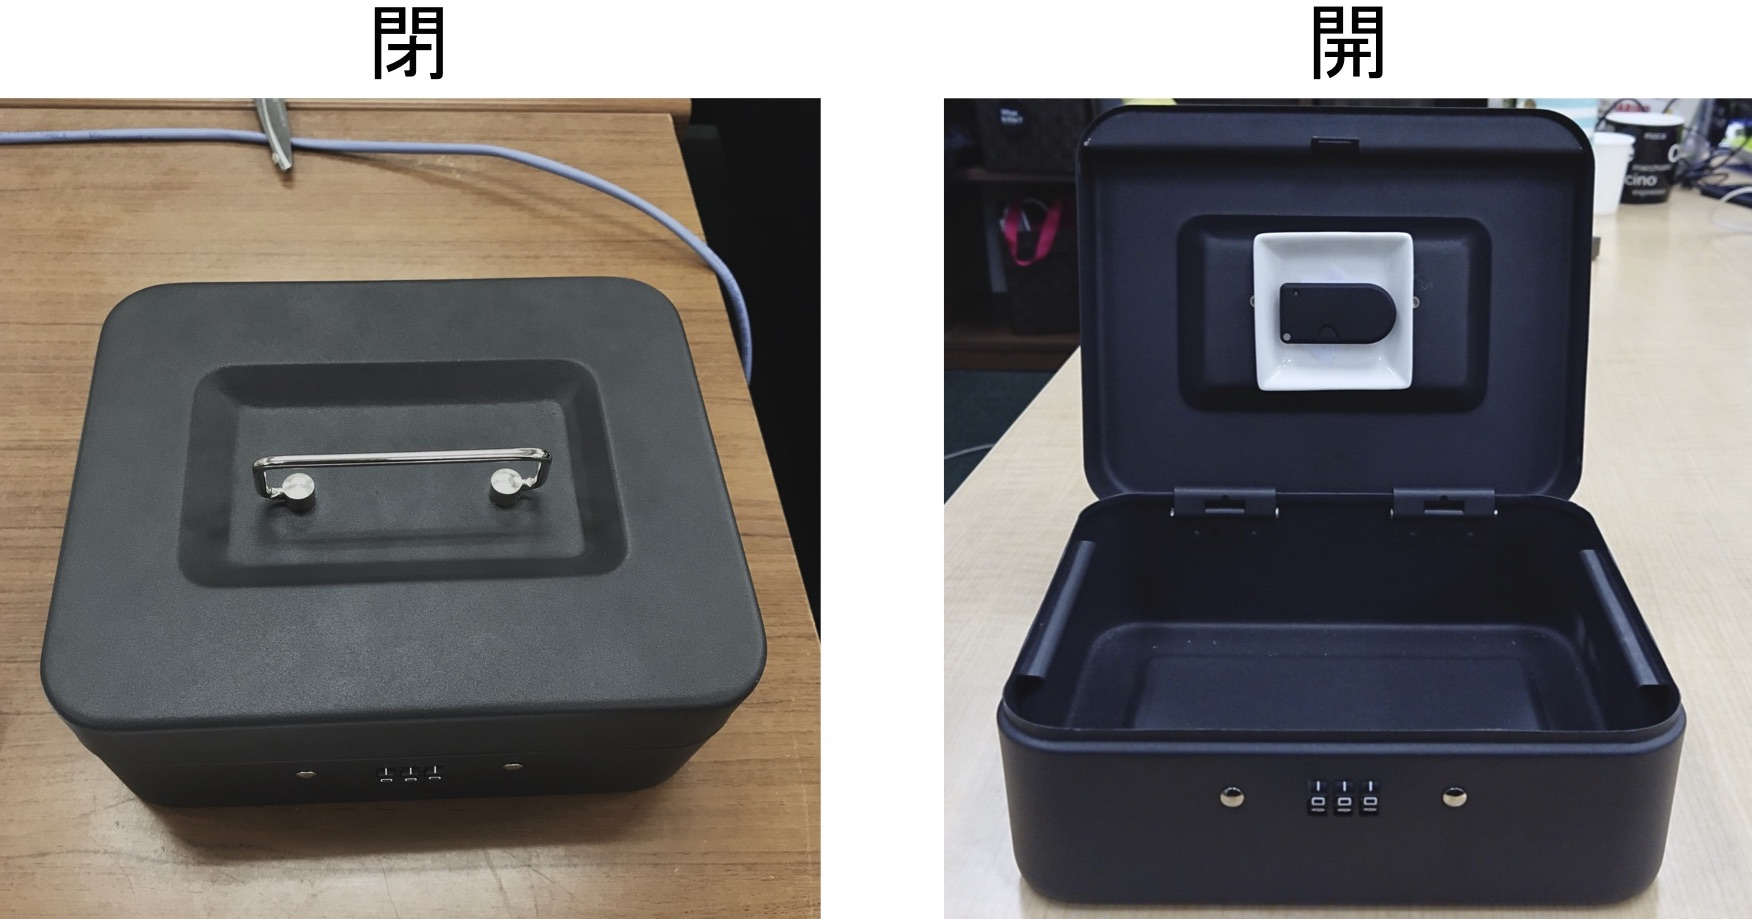
\includegraphics[width=10cm]{images/chapter3/kinkoW.jpg}
    \caption{金庫の状態と設置したBLEビーコン}
    \label{safe}
\end{figure}


\begin{figure}[H]
    \centering
    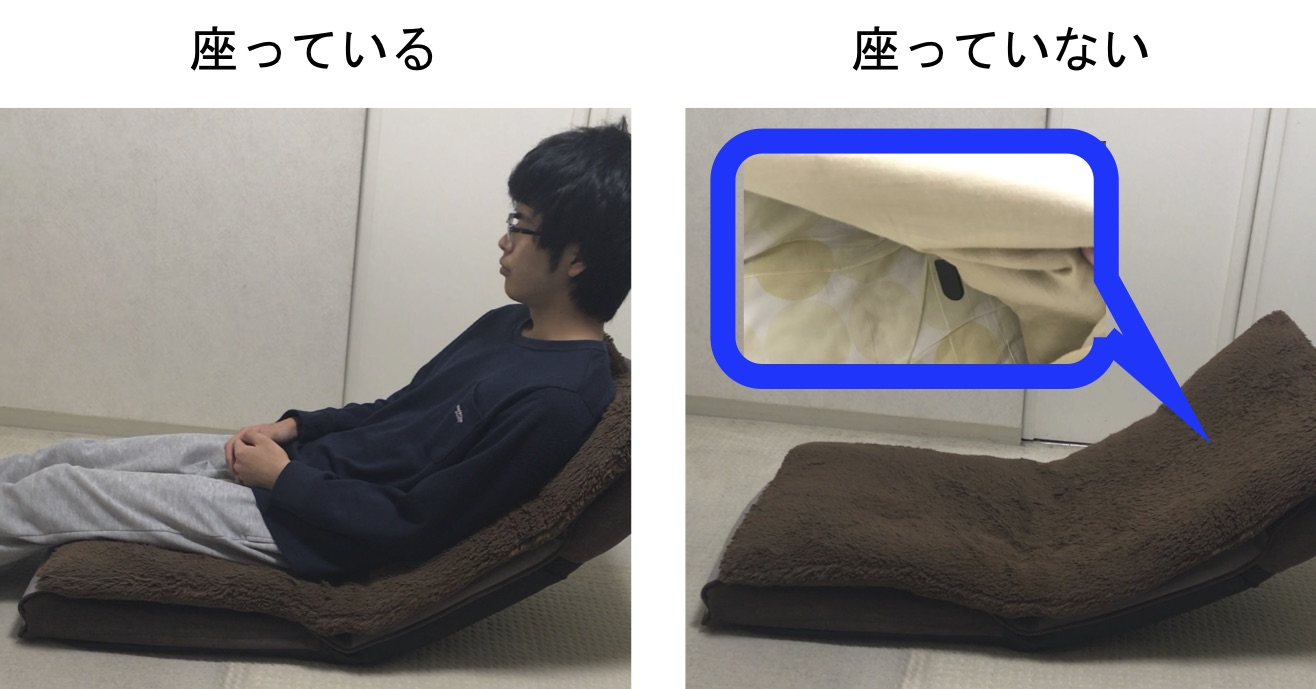
\includegraphics[width=10cm]{images/chapter3/zaisuW.jpg}
    \caption{座椅子の状態と設置したBLEビーコン}
    \label{chair}
\end{figure}


\begin{figure}[tbh]
    \centering
    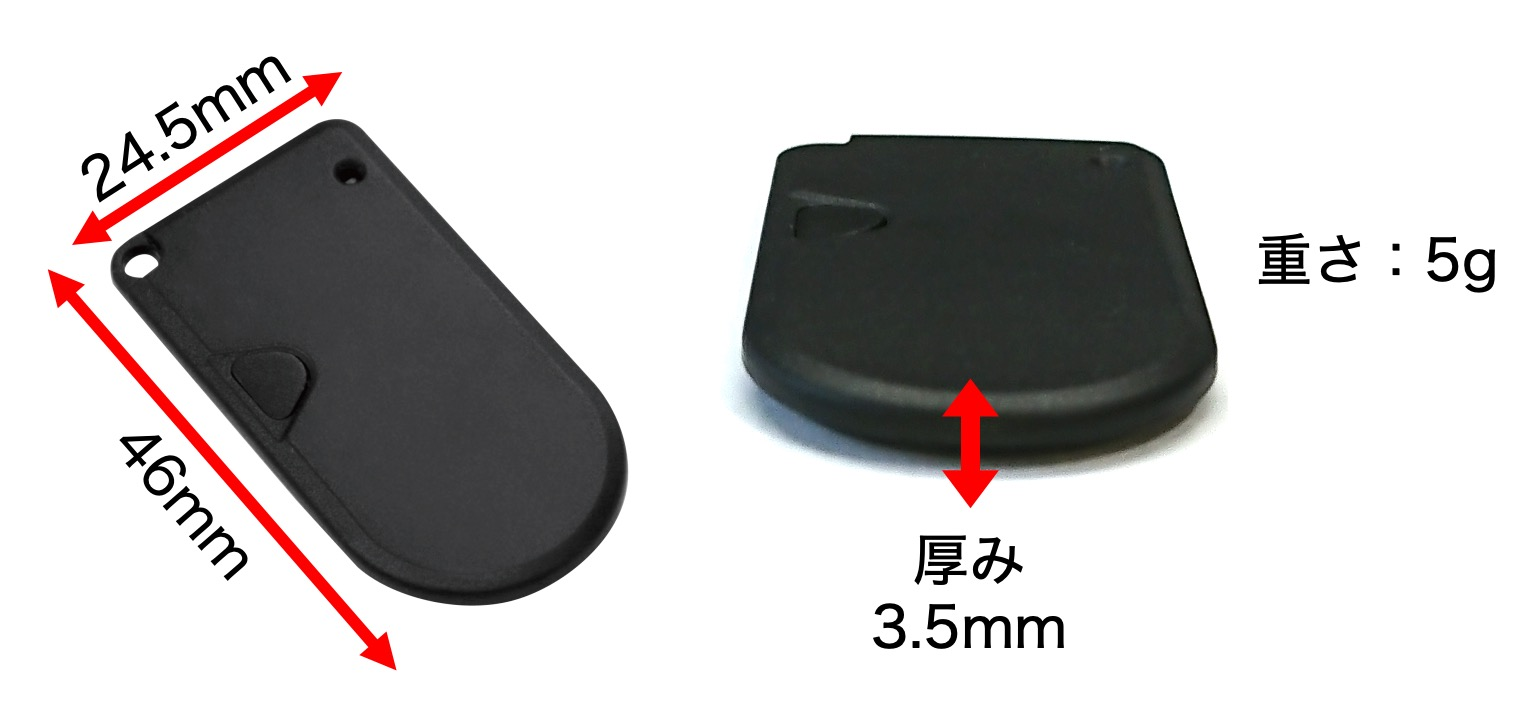
\includegraphics[width=10cm]{images/chapter3/BLE_beacon_info.jpg}
    \caption{BLEビーコン}
    \label{beacon}
\end{figure}


%ーーーーーーーーーーーーーーーーーーーーーーーーーーーーーーーーーーーーーーーーーーーーーーーーー
%ーーーーーーーーーーーーーーーーーーーーーーーーーーーーーーーーーーーーーーーーーーーーーーーーー


\section{BLEビーコンの取り付け位置の検討と設定}
本研究では,モノの状態が変化した際のBLEビーコンの電波強度変化をもとに状態推定を行う.
そのため,BLEビーコンはその変化が一番大きくなる位置に設置する必要がある.
例えば,箱型で蓋の開閉を行う金庫のようなものであれば,BLEビーコンを箱内部の底に設置する場合と,蓋の裏に設置する場合が考えられる(図\ref{adapter}).
また,モノの材質によっては電波を通しやすく,状態変化しても電波強度に大きな変化が現れないモノもある.
そこで,図\ref{adapter}の右側に示すようにBLEビーコンに対して指向性アダプタを取り付ける.
この指向性アダプタとは,図\ref{adapter_only}に示す金属や陶器でできたパラボラアンテナのような形状の物を指す.
取り付けた際の効果として,電波が拡散せず収束して一方向のみへ飛ぶようになり,状態変化によって電波強度に大きな変化が現れるようになる.


\begin{figure}[H]
    \centering
    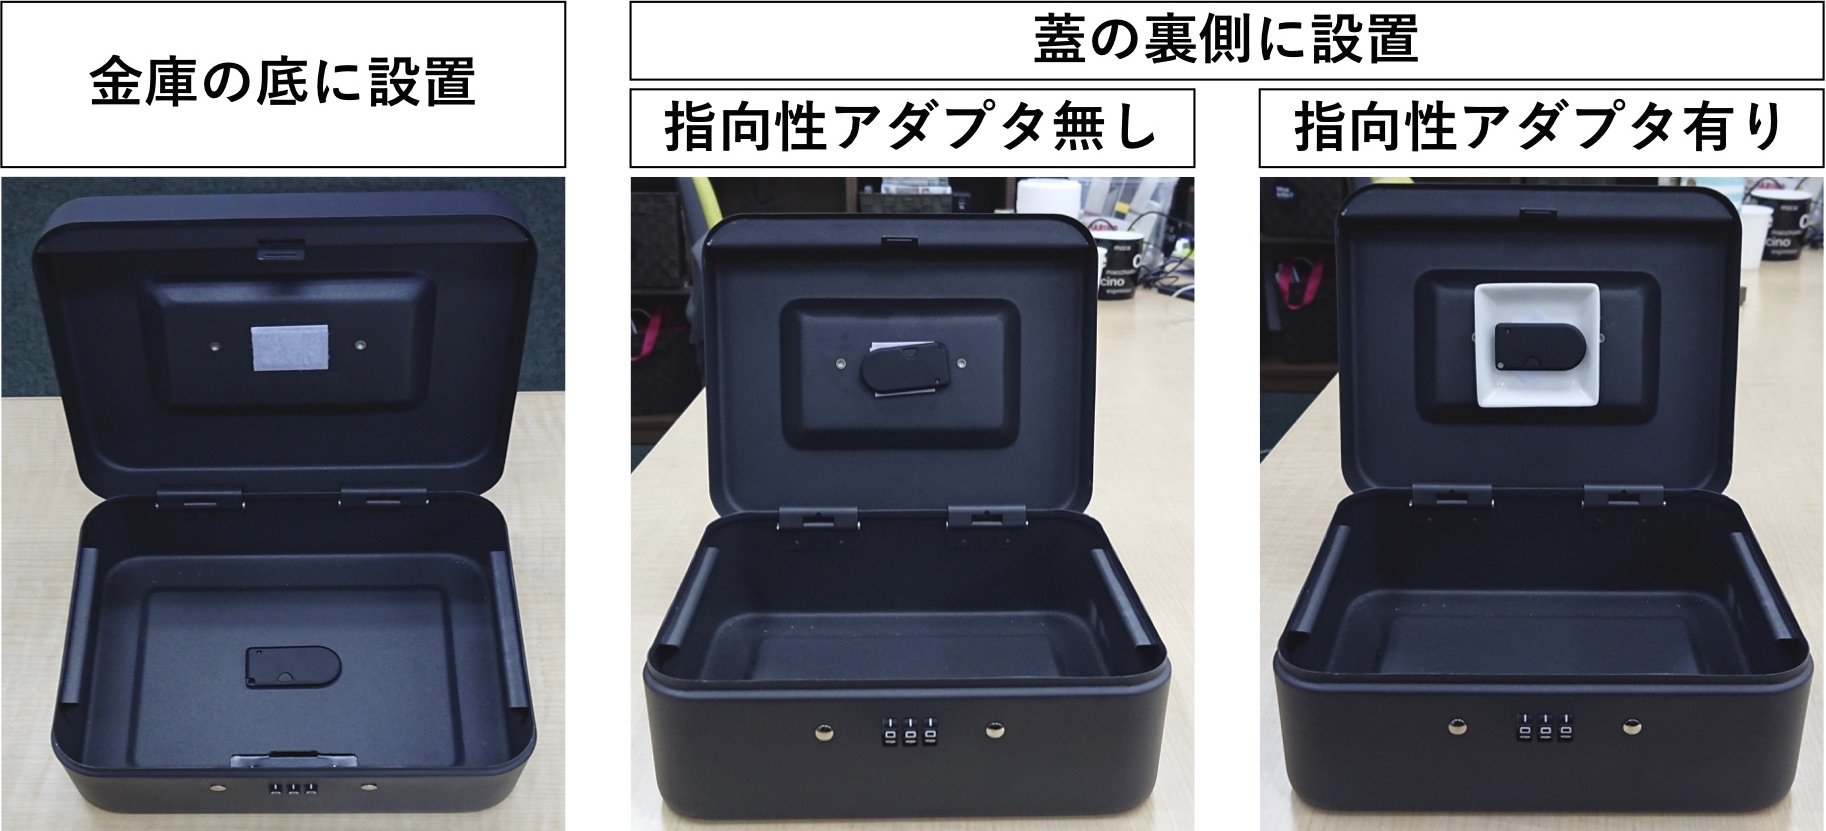
\includegraphics[width=12cm]{images/chapter3/adapta_compare.jpg}
    \caption{BLEビーコンの設置場所と指向性アダプタ}
    \label{adapter}
\end{figure}


\begin{figure}[H]
    \centering
    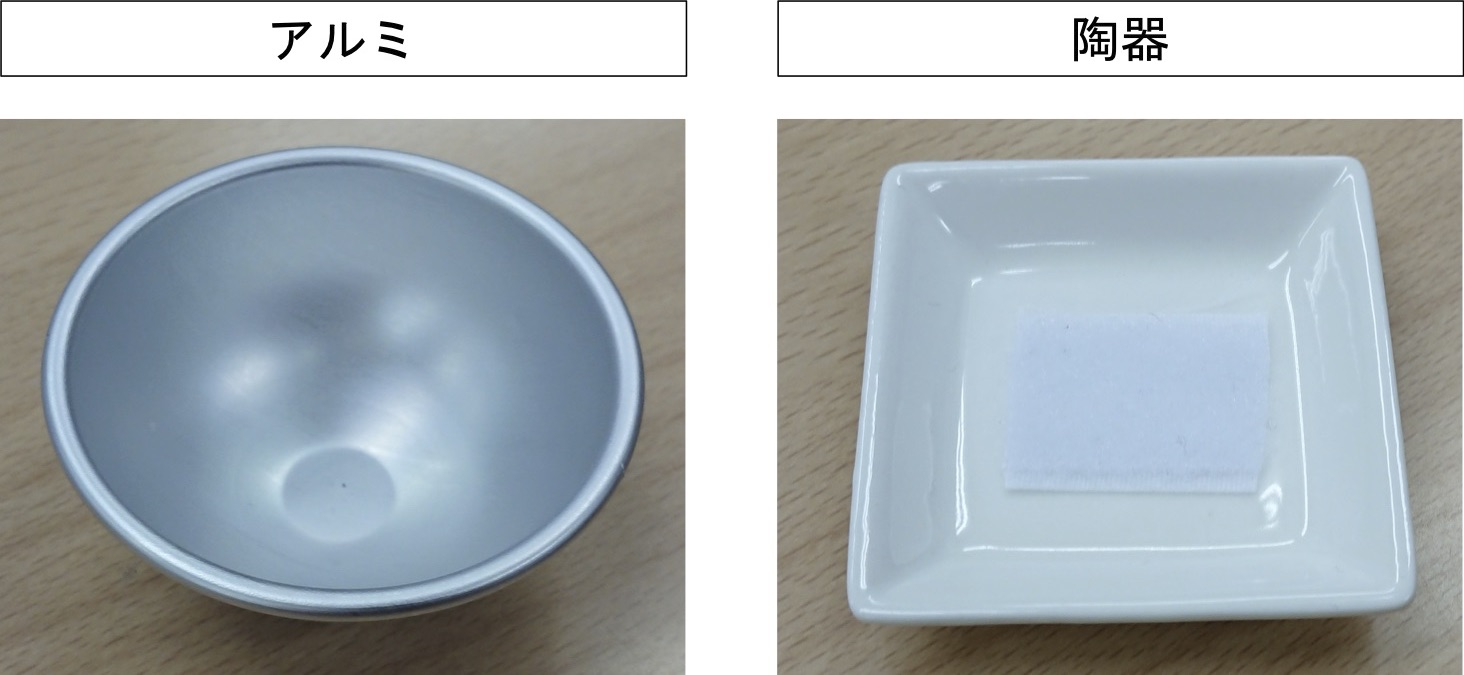
\includegraphics[width=12cm]{images/chapter3/adapta.jpg}
    \caption{本研究で使用した指向性アダプタ}
    \label{adapter_only}
\end{figure}


図\ref{transform-data}にそれぞれの取り付け方による金庫開閉時の電波強度の波形を示す.
この図にはそれぞれ開いている状態と閉じている状態の正解ラベルをつけている.
BLEビーコンを金庫内部の底につけた場合にはあまり大きな変化は見られず,蓋の裏側にBLEビーコンを設置した場合では大きな変化が見られる.
さらに,指向性アダプタをつけた場合には,よりくっきりと電波強度に差が現れる.
このように,状態推定対象物に合わせてBLEビーコンの取り付け方を工夫し,状態推定の高精度化を図る.

本研究では受信機としてスマートフォンを使用するため,専用のAndroidアプリケーションを作成し,電波強度の情報を収集する.
その際,BLEビーコンを識別するためのUUID,major,minorをBLEビーコンを設置する対象と紐付けし,どのBLEビーコンの値がどの対象物のモノなのか把握できるようにしている.
また,小さな変化も検知できるようにBLEビーコンの電波送信設定は,送信強度は0dBm,送信間隔は100msと設定している.

\begin{figure}[H]
    \centering
    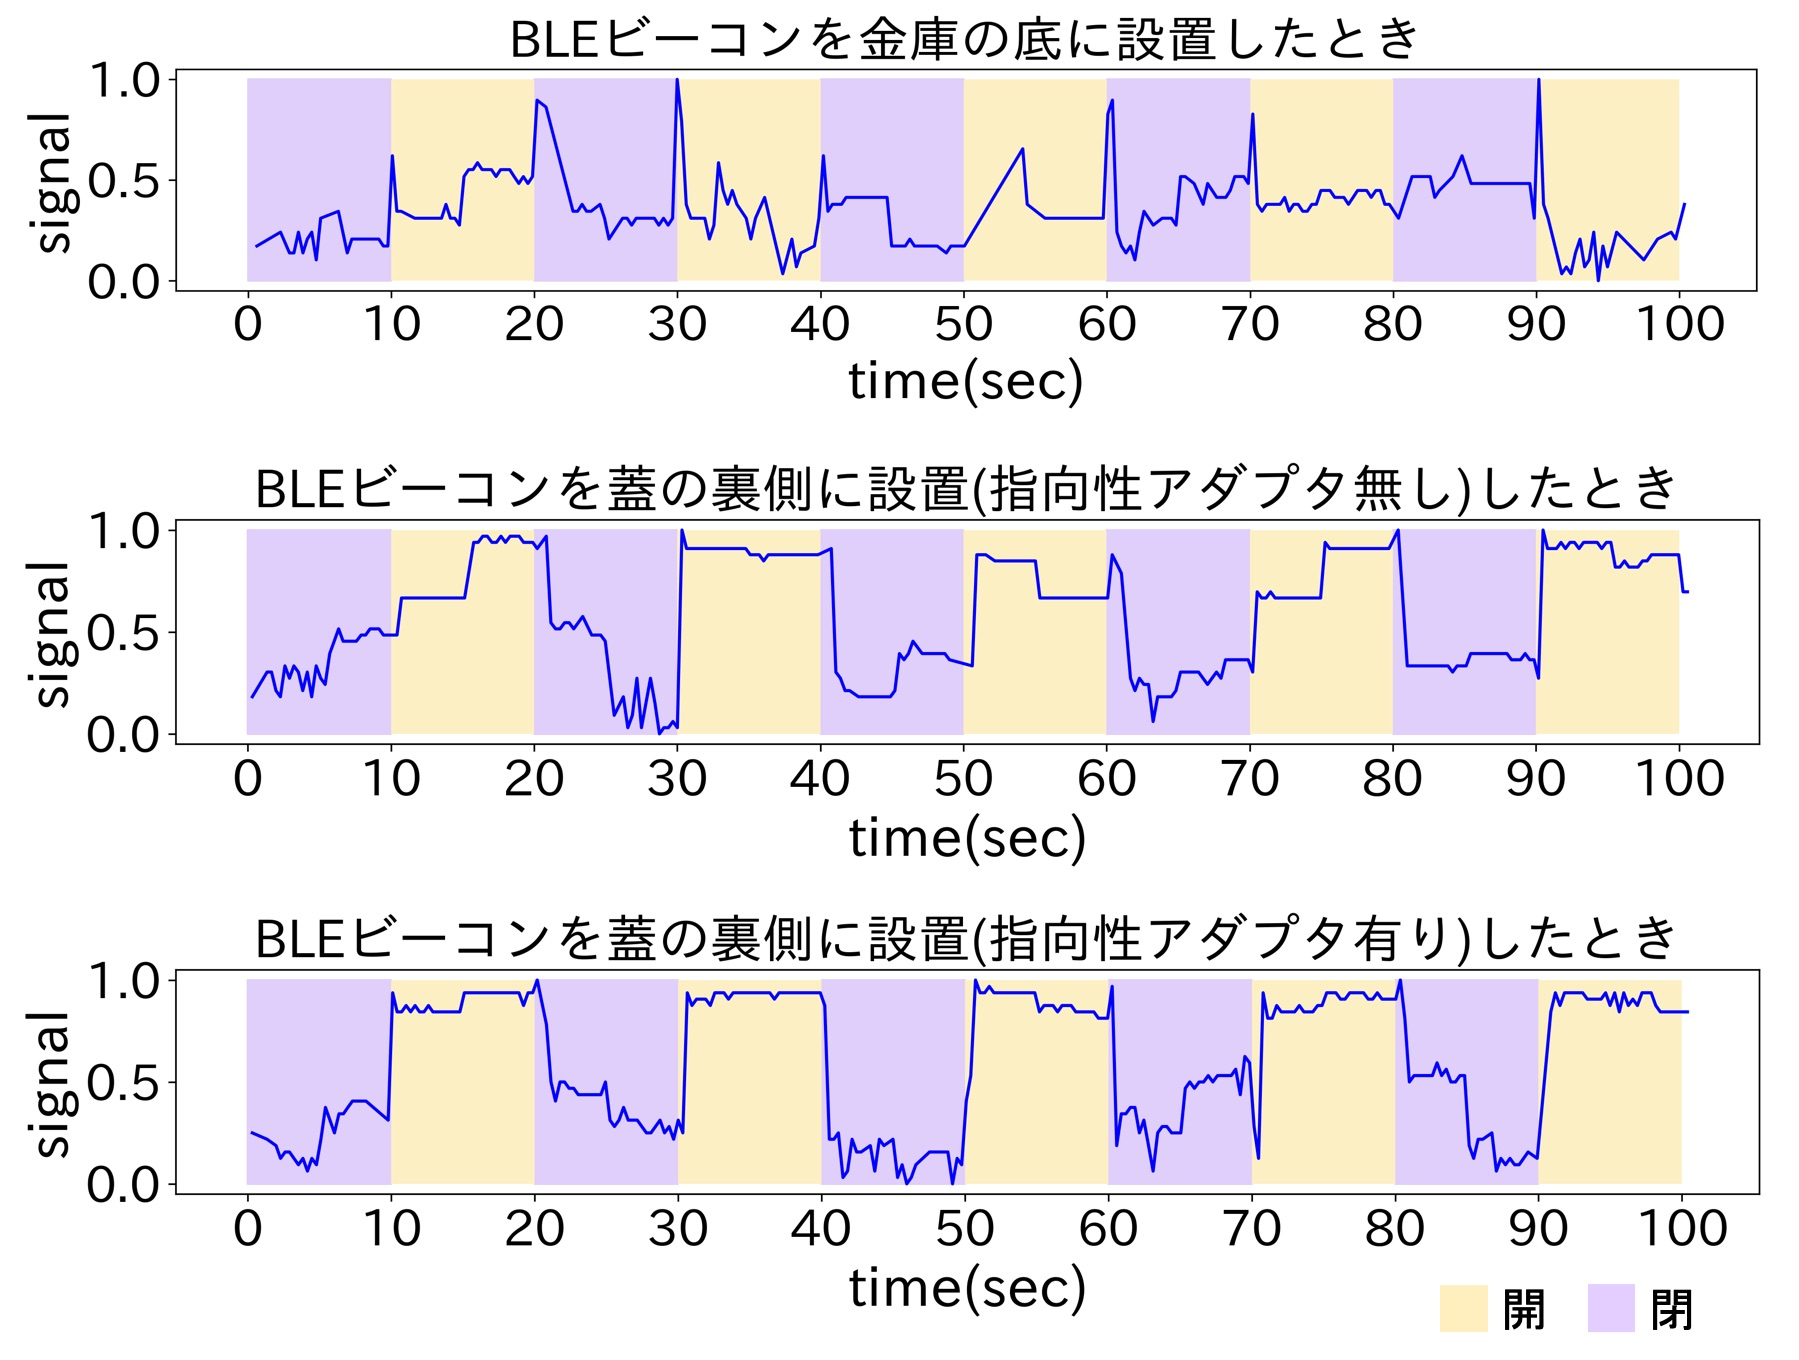
\includegraphics[width=14cm]{images/chapter3/in-out.jpg}
    \caption{BLEビーコン取り付け位置ごとの電波強度変化}
    \label{transform-data}
\end{figure}


%ーーーーーーーーーーーーーーーーーーーーーーーーーーーーーーーーーーーーーーーーーーーーーーーーー
%ーーーーーーーーーーーーーーーーーーーーーーーーーーーーーーーーーーーーーーーーーーーーーーーーー


\section{状態推定アルゴリズム}

\begin{figure}[tbh]
    \centering
    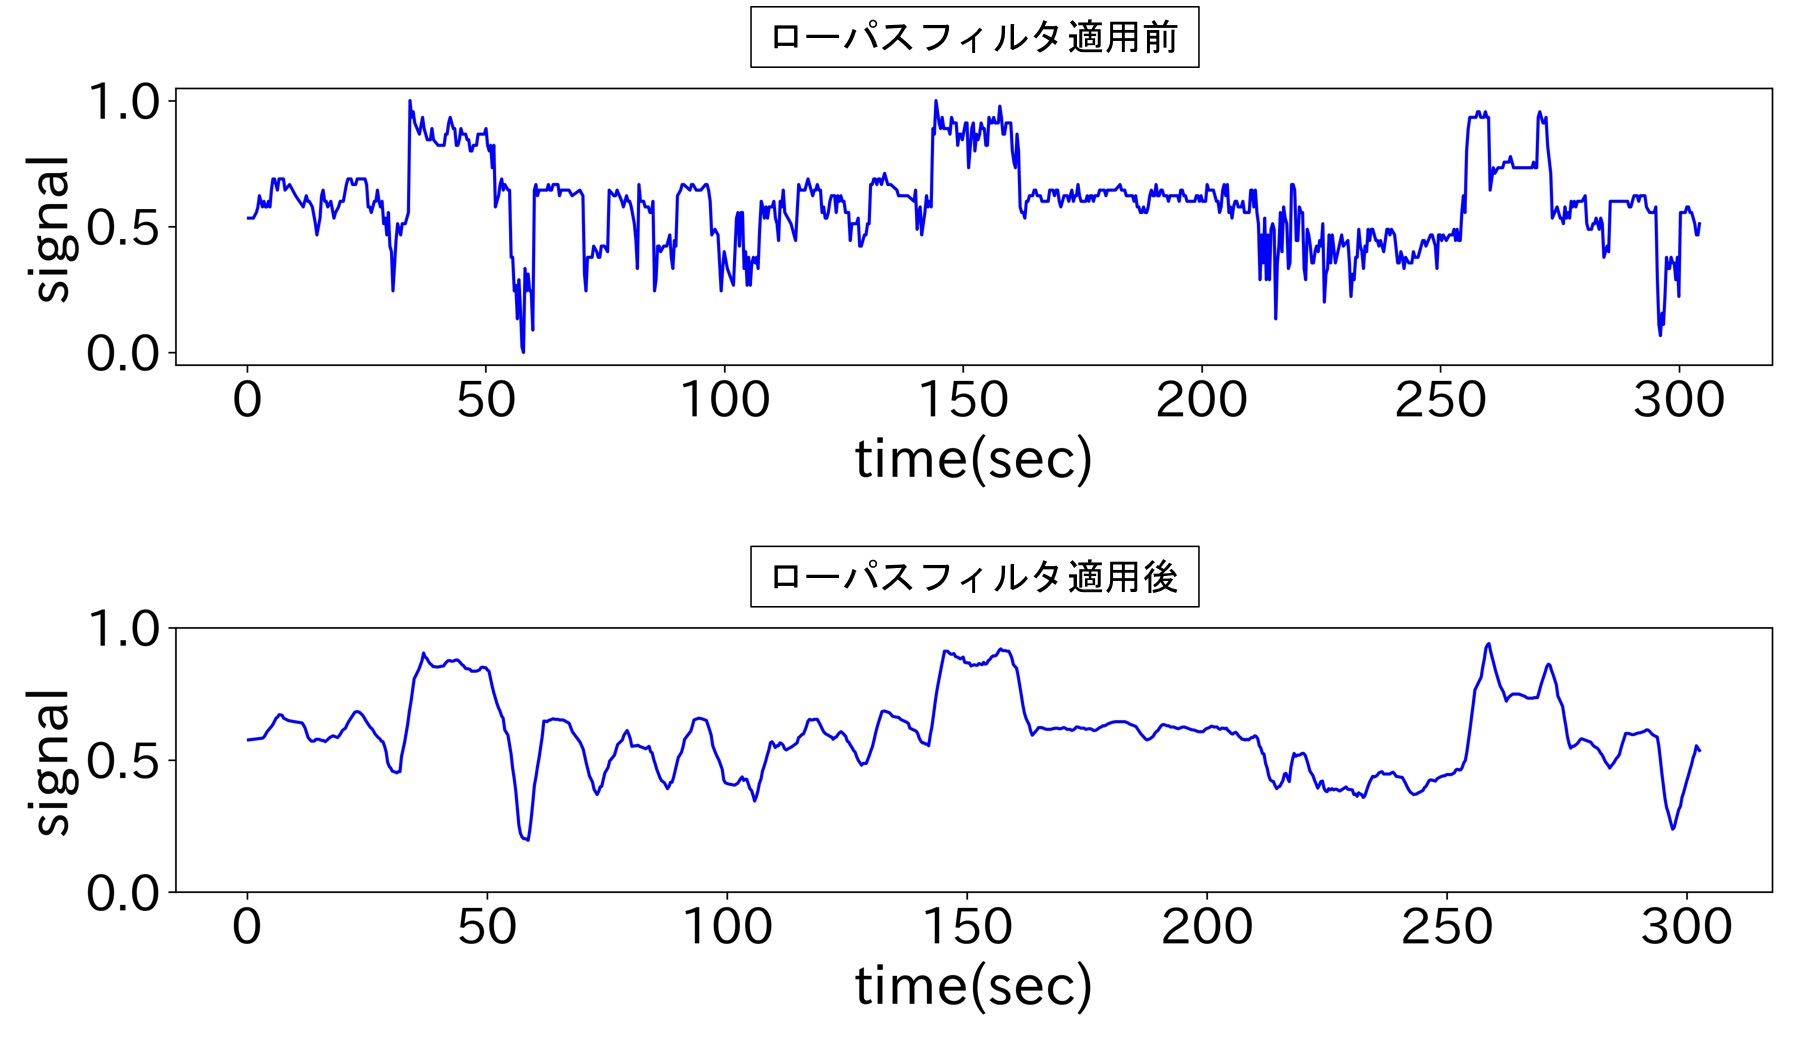
\includegraphics[width=14cm]{images/chapter3/lowpath_compare.jpg}
    \caption{ノイズ軽減処理前後の波形比較}
    \label{bank-opcl}
\end{figure}

本手法ではBLEビーコンから発せられる電波を300msの間隔で受信し,その受信電波強度の値から状態を推定する.
このとき,取得したデータをそのまま使用すると,ノイズによる影響を受けてしまい正確に推定を行えない.
そこで,取得したデータに対して複数の処理を適用し,ノイズの軽減を図る.
ノイズを軽減するための処理として,本手法ではローパスフィルタと正規化を使用する.
このとき,ローパスフィルタには10個のサンプル,つまり3秒分のデータを用いる.
図\ref{bank-opcl}に金庫の蓋を開閉した際の電波強度変化グラフと,ノイズ軽減処理の結果を示す.

% \subsection{安定センシング区間}
本手法では推定対象物の移動も考慮する.
しかし,物体が状態変化をせず移動した場合や人の往来,BLEビーコンの発する電波の揺らぎなどによって受信電波強度が安定しない場合がある.
% しかし,物体が状態変化をせず移動した場合,電波強度は徐々に変化するため閾値を用いた単純な推定では誤判定が起きてしまう.
そこで,梶ら\cite{sensing-area}が提案している安定センシング区間という概念を利用し,推定精度の高精度化を図る.
安定センシング区間とは,一定時間以上センシングが安定して行えている区間を指す.
本研究ではある値に着目した際に,その値が基準となる値の上限・下限閾値の範囲内であり,かつ一定時間以上経過している区間がそれにあたる.

図\ref{nomal-data}はBLEビーコンを遮蔽物のない環境で測定した電波強度のグラフであるが,ここからBLEビーコンの電波は電波強度が周期的に変化しているのがわかる.
このBLEビーコン特有の周期的な電波強度変化により安定センシング区間の判定が不安定になるため,上限・下限閾値は使用するBLEビーコンや推定対象物の特徴に合わせて設定を行う.
もし,閾値を超えた場合は,超える直前の受信電波強度の値に±Xした値を新しい閾値として設定する.
これにより推定対象物が移動しても状態推定が可能となる.

\begin{figure}[tbh]
    \centering
    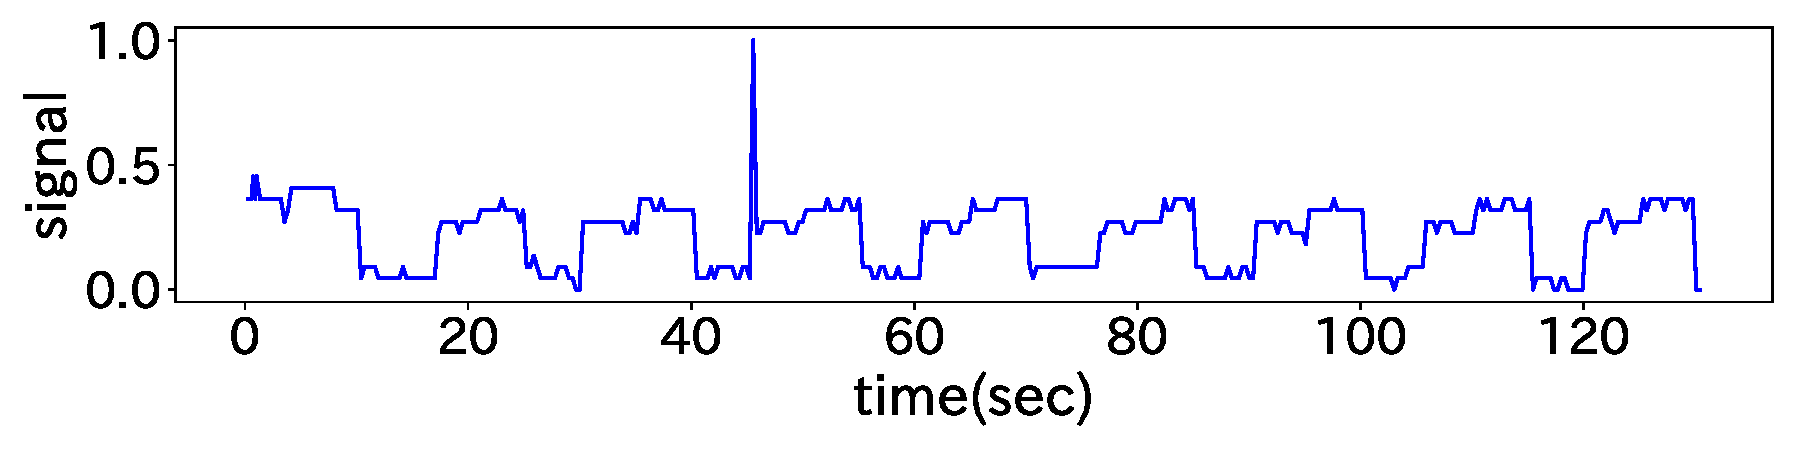
\includegraphics[width=14cm]{images/chapter3/bokoboko.pdf}
    \caption{BLEビーコンを遮蔽物のない状態で測定した電波強度グラフ}
    \label{nomal-data}
\end{figure}

% \subsection{状態変化の推定}
安定センシング区間の判定が終わったら,見つけた各区間がポジティブな状態か,ネガティブな状態か判定を行う.
ポジティブな状態とはBLEビーコンが外に出ていて電波の受信がしやすく、電波強度の値が大きい状態を指す.
具体的には金庫の開閉であれば開いてる状態である.
ネガティブな状態とはBLEビーコンが外に出ておらず電波の受信が難しく、電波強度の値が小さい状態を指す.
具体的には金庫の開閉であれば閉じてる状態である.
判定は,各安定センシング区間の受信電波強度の平均値が,全受信電波強度の中央値に0.1を足した値より大きいか小さいかで行う.


\section{評価実験}
本稿で提案した手法の推定精度を確かめるため,冷蔵庫,金庫,座椅子へBLEビーコンを設置し評価実験を行った.
実験条件として,評価はBLEビーコンと受信機の間に障害物が存在しない理想環境で実施し,推定結果と正解ラベルから正答率を算出して行った.
また,安定センシング区間の概念の効果を実証するため,金庫と座椅子については移動を考慮した評価を行った.


\subsection{実験端末の選定}

\begin{figure}[tbh]
    \centering
    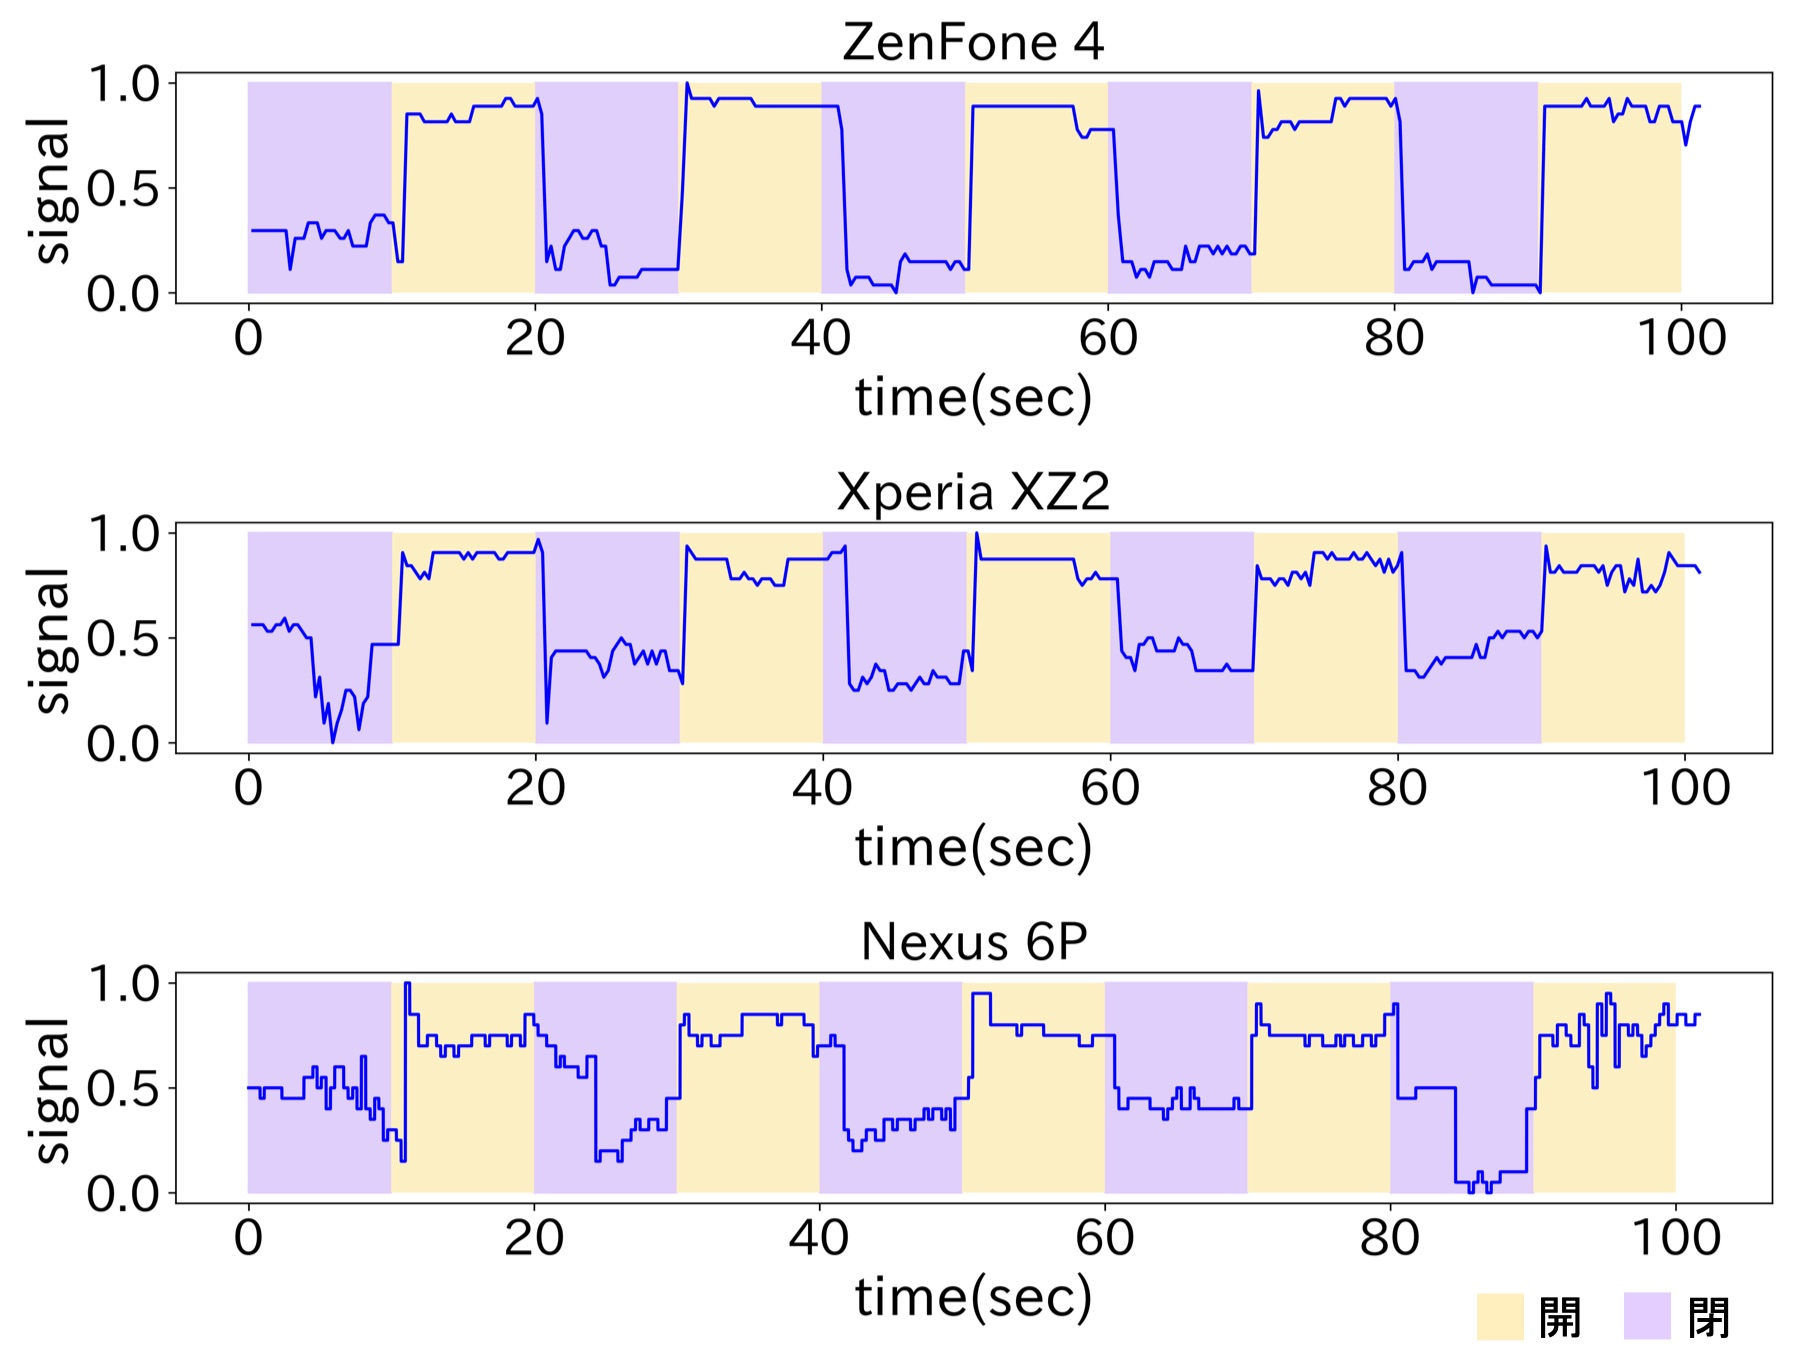
\includegraphics[width=14cm]{images/chapter3/mix.jpg}
    \caption{機種ごとの精度比較}
    \label{multi-data}
\end{figure}

Bluetoothのセンサ精度は端末ごとに異なるため,実験に用いる端末は変化を正しく捉えられる端末を使うのが望ましい.
そこでAndroid端末を3機種用意し,同一環境下で金庫の蓋の開閉を行い測定精度の比較を行った.
今回用意した端末はXperia XZ2,Nexus 6P,ZenFone 4である.
金庫開閉時の電波強度変化を各端末で収集し,その波形を比較した結果を図\ref{multi-data}に示す.
図の紫色の部分は蓋が閉まっている状態を黄色の部分は蓋が開いている状態を示している.
3機種の精度を比較した結果,Nexus 6Pでは全体的に小さなノイズが発生しているがZenFone 4とXperia XZ2ではそれが少ない.
また,Xperia XZ2とNexus 6Pは測定開始直後は測定値が安定せず正しく変化を捉えられていない.

本手法では電波強度の急激な変化と安定センシング区間の判定が重要となるため,測定ノイズが少なく電波を正確に捉えられる必要がある.
そこで,この3機種のうち一番ノイズが少なかったZenFone 4を実験で用いる受信機として採用した.
また,本研究では金庫などの移動を伴う比較的小さなモノにもBLEビーコンを取り付けるため,使用するBLEビーコンはできるだけ小さい方が望ましい.
そのためBLEビーコンは軽量・小型という理由からフォーカスシステムズ社のFCS1301(図\ref{beacon})を使用した.


\subsection{冷蔵庫の開閉における推定精度の測定}
図\ref{freezer},図\ref{refrigerator_position}のようにBLEビーコンと受信機を設置した冷蔵庫で評価実験を行った.
実験は日常の使用を模倣し,冷蔵庫のドアを開けて中からペットボトルを取り出し,ドアを閉めるという動作をランダムな間隔で行い,その状態変化を捉えられるか評価を行った.
日常使いにおいて冷蔵庫を開ける動作時間は約7秒程度であるため本実験でもそれを模倣し,閉めている状態はランダムに1分から5分程度の時間を設けた.
このとき,冷蔵庫が開いている状態も推定可能にするため安定センシング区間を判定する閾値はそれぞれ,値の閾値を±0.23,時間の閾値を2秒に設定した.
また,BLEビーコンを扉の棚へ置いただけではあまり電波強度に変化が見られなかったため,電波強度の変化を大きくさせるよう3.2章で述べた指向性アダプタを取り付けた.
推定結果を図\ref{refrigerator_graph}に,正解率の一覧を表\ref{refrigerator_fig}に示す.
図\ref{refrigerator_graph}の白色の範囲は安定センシング区間ではない状態を,緑色の範囲はネガティブな状態(ドアが閉まっている状態)を,赤色の範囲はポジティブな状態(ドアが開いている状態)を示している.

同様の実験を3回行った結果1回だけ不正解があり,試行回数をもとにした状態推定精度は98.0\%,推定ラベルのうち正しく推定できた時間をもとにした状態推定精度は99.2\%となった.


\begin{figure}[tbh]
    \centering
    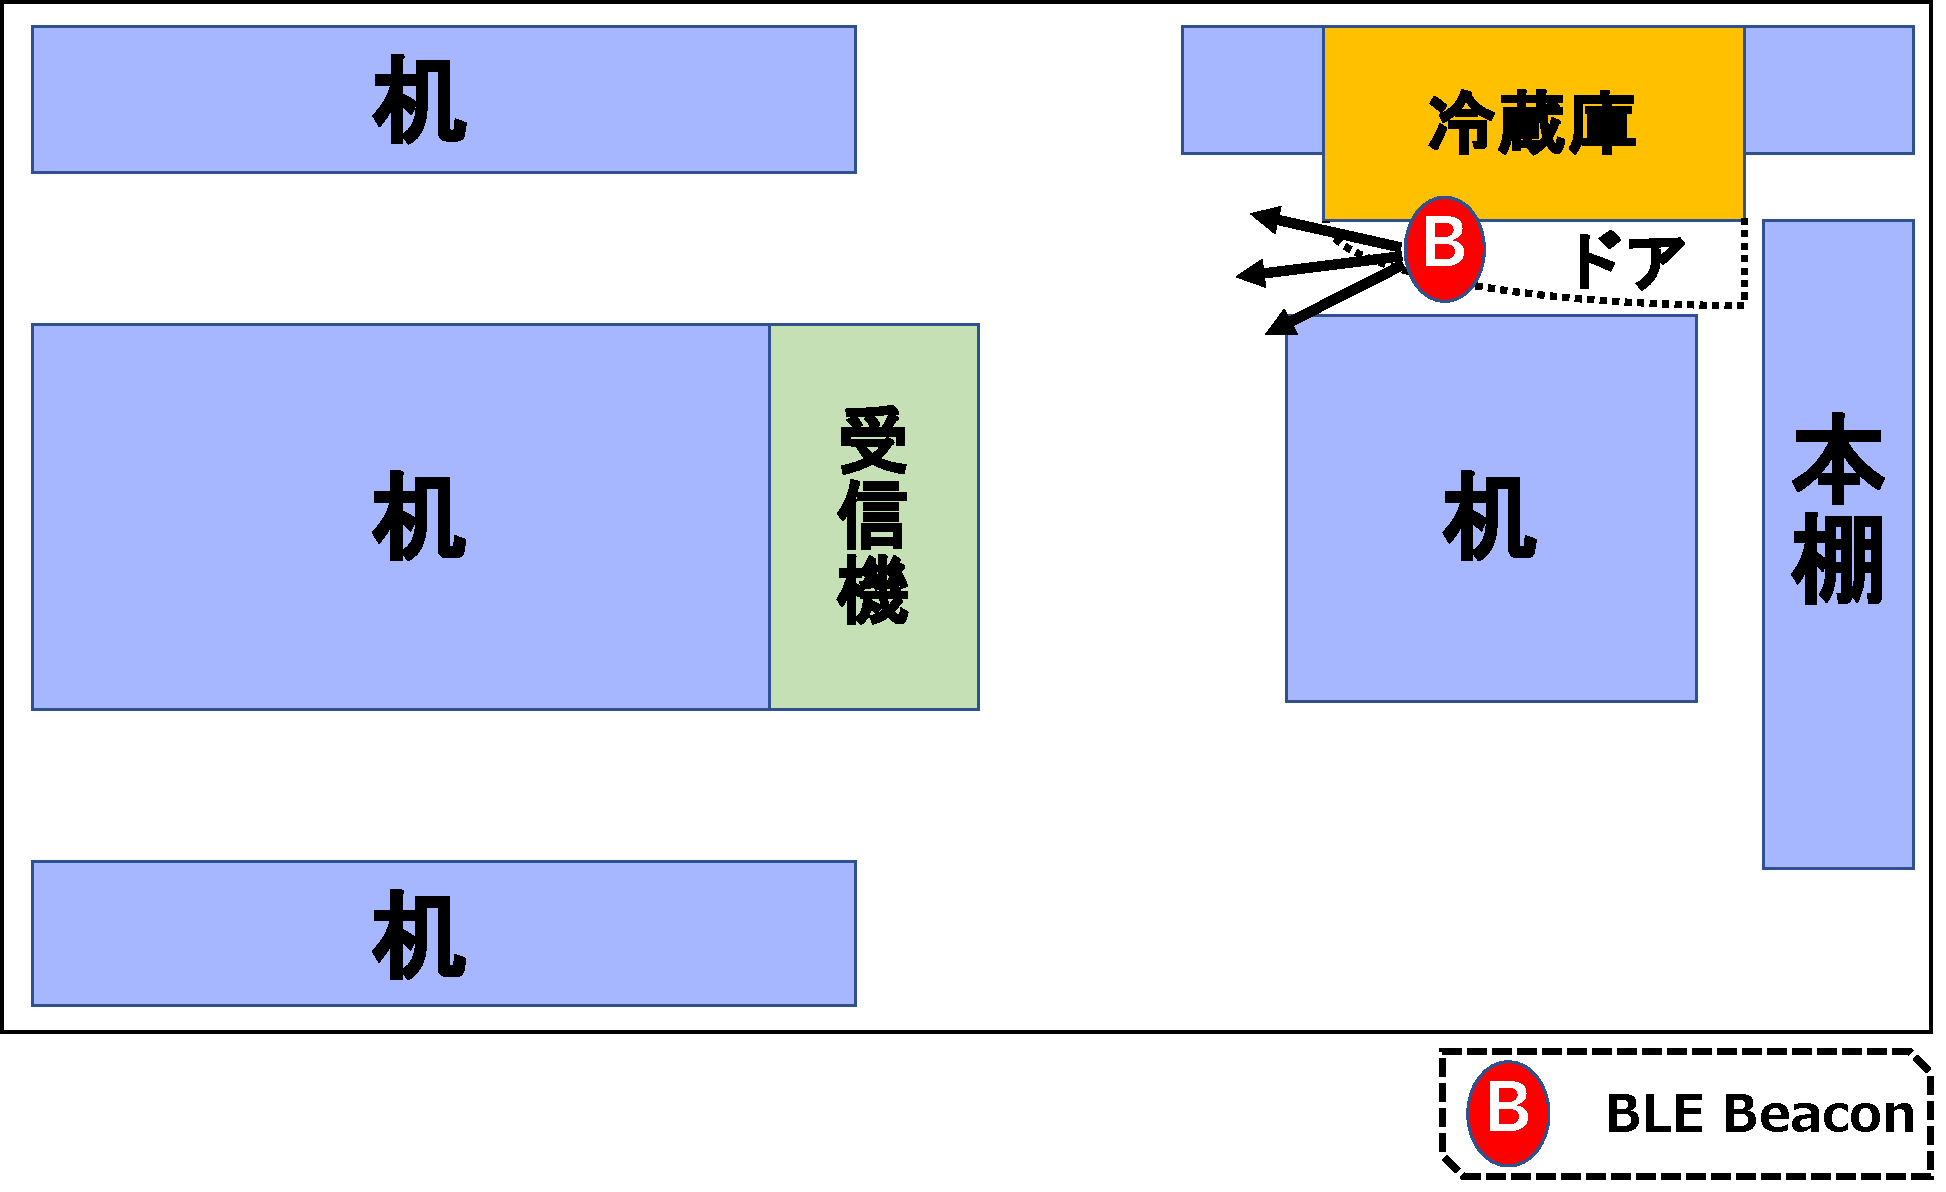
\includegraphics[width=10cm]{images/chapter3/refrigerator_position.pdf}
    \caption{冷蔵庫と受信機の位置関係図}
    \label{refrigerator_position}
\end{figure}


\begin{figure}[tbh]
    \centering
    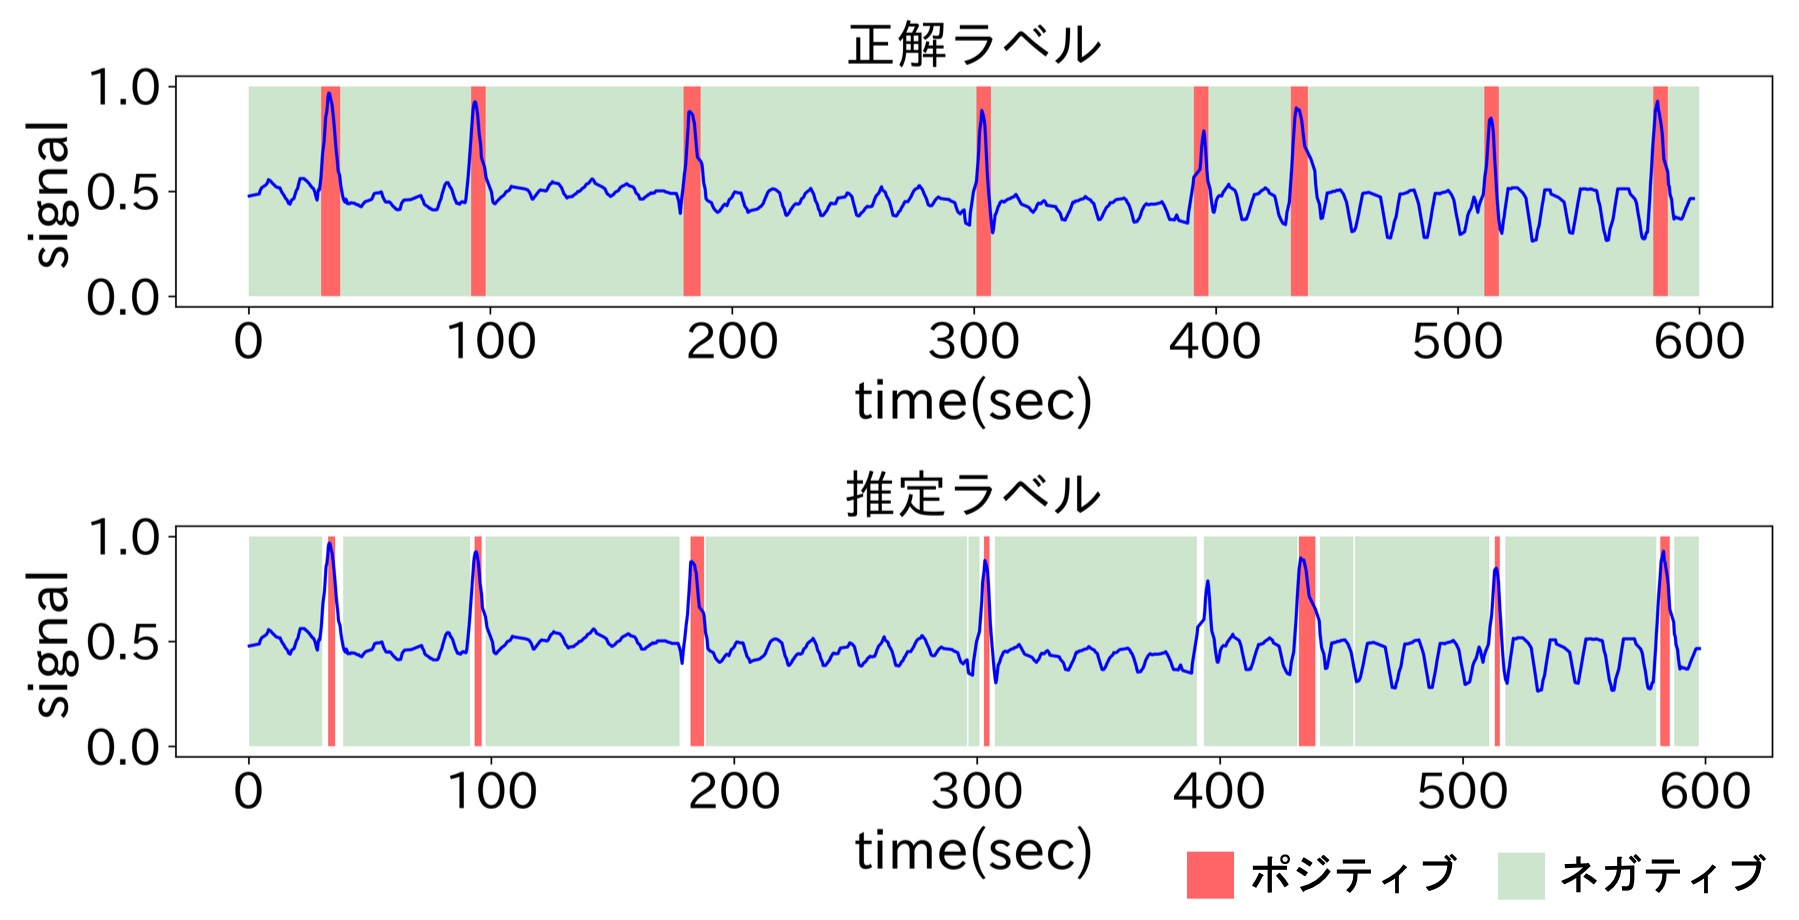
\includegraphics[width=14cm]{images/chapter3/refrigerator_graph.jpg}
    \caption{冷蔵庫の状態推定結果グラフ}
    \label{refrigerator_graph}
\end{figure}


\begin{table}[tbh]
    \begin{center}
        \caption{冷蔵庫の開閉における状態推定精度}
        \label{refrigerator_fig}
        \begin{tabular}{|c|c|c|c|} \hline
        試行回数 & 正答率 & 正解数 & 不正解数 \\ \hline
        1 & 94.1\% & 16 & 1 \\ \hline
        2 & 100\% & 17 & 0 \\ \hline
        3 & 100\% & 17 & 0 \\ \hline \hline
        回数でみた累計正解率 & \multicolumn{3}{c|}{98.0\%} \\ \hline \hline
        推定ラベルの正解割合 & \multicolumn{3}{c|}{99.2\%} \\ \hline
        \end{tabular}
    \end{center}
\end{table}


\subsection{金庫の開閉における推定精度の測定}
図\ref{safe},図\ref{kinko_position}のようにBLEビーコンを設置した金庫と受信機を設置して評価実験を行った.
金庫は図\ref{kinko_position}内に示したの3つの場所でそれぞれ蓋の開閉を行い,推定中にモノの移動が行われても状態推定が可能かを確かめた.
このとき,金庫を開けている時間は約20秒程度であり,閉めた状態はランダムに30秒から2分程度継続させた.
また,安定センシング区間を判定する閾値はそれぞれ,値の閾値を±0.23,時間の閾値を4.5秒に設定した.
推定結果を図\ref{kinko_graph}に,正解率の一覧を表\ref{kinko_fig}に示す.
図\ref{kinko_graph}の白色の範囲は安定センシング区間ではない状態を,緑色の範囲はネガティブな状態(蓋が閉まっている状態)を,赤色の範囲はポジティブな状態(蓋が開いている状態)を示しており,図中の番号は図\ref{kinko_position}内の番号と対応している.

同様の実験を3回行った結果,試行回数をもとにした状態推定精度は100\%,推定ラベルのうち正しく推定できた時間をもとにした状態推定精度は93.8\%であった.

\begin{figure}[tbh]
    \centering
    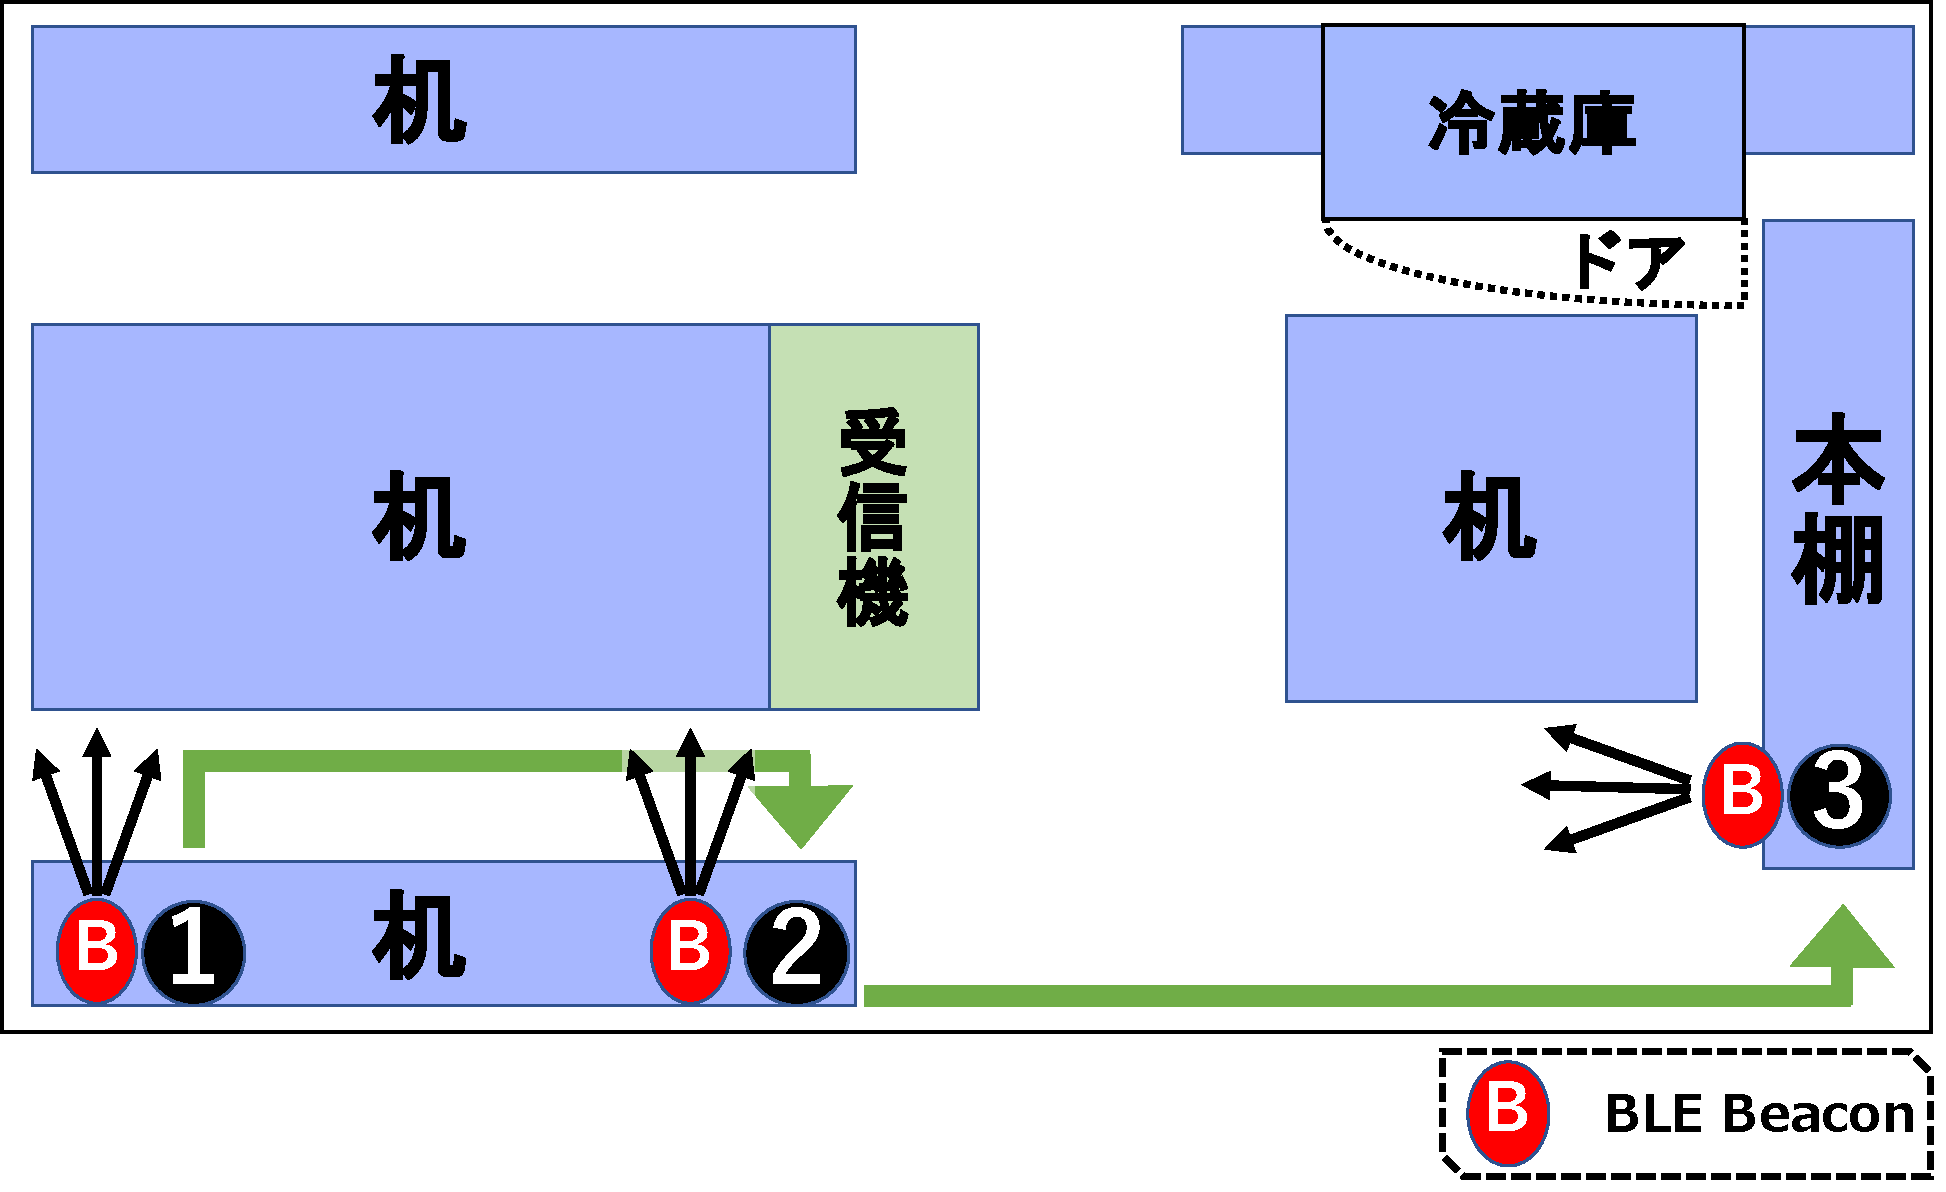
\includegraphics[width=10cm]{images/chapter3/kinko_position_fig.pdf}
    \caption{金庫と受信機の位置関係図}
    \label{kinko_position}
\end{figure}

\begin{figure}[tbh]
    \centering
    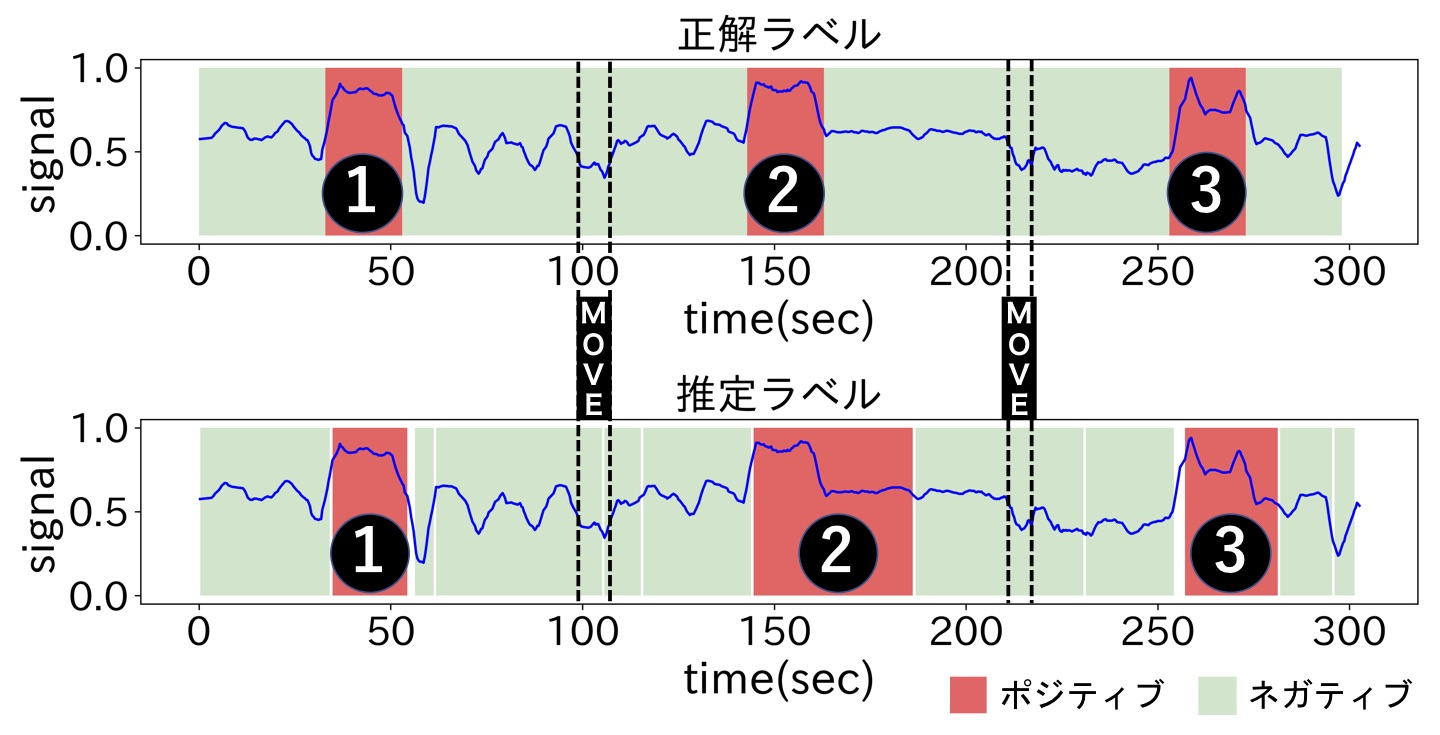
\includegraphics[width=14cm]{images/chapter3/kinko_graph.jpg}
    \caption{金庫の状態推定結果グラフ}
    \label{kinko_graph}
\end{figure}

\begin{table}[tbh]
    \begin{center}
        \caption{金庫の開閉における状態推定精度}
        \label{kinko_fig}
        \begin{tabular}{|c|c|c|c|} \hline
        試行回数 & 正答率 & 正解数 & 不正解数 \\ \hline
        1 & 100\% & 7 & 0 \\ \hline
        2 & 100\% & 7 & 0 \\ \hline
        3 & 100\% & 7 & 0 \\ \hline \hline
        回数でみた累計正解率 & \multicolumn{3}{c|}{100\%} \\ \hline \hline
        推定ラベルの正解割合 & \multicolumn{3}{c|}{93.8\%} \\ \hline
        \end{tabular}
    \end{center}
\end{table}


\subsection{座椅子の着座における推定精度の測定}
図\ref{chair},図\ref{zaisu_position}のようにBLEビーコンを設置した座椅子と受信機を設置して評価実験を行った.
動作の流れとして,1の位置で着座を行った後,2の場所に座椅子を移動させて再度着座を行った.
座椅子に座っている時間として30秒から1分30秒程度を,座っていない時間として30秒から2分程度を設定した.
また,安定センシング区間を判定のための閾値はそれぞれ,値の閾値は±0.235,時間の閾値は5秒に設定した.
推定結果を図\ref{chair_graph}に,正解率の一覧を表\ref{chair_fig}に示す.
図\ref{chair_graph}の白色の範囲は安定センシング区間ではない状態を,緑色の範囲はネガティブな状態(人が座っている状態)を,赤色の範囲はポジティブな状態(人が座っていない状態)を示しており,図中の番号は図\ref{zaisu_position}内の番号と対応している.

同様の実験を3回行った結果,試行回数をもとにした状態推定精度は100\%,推定ラベルのうち正しく推定できた時間をもとにした状態推定精度は98.9\%であった.


\begin{figure}[tbh]
    \centering
    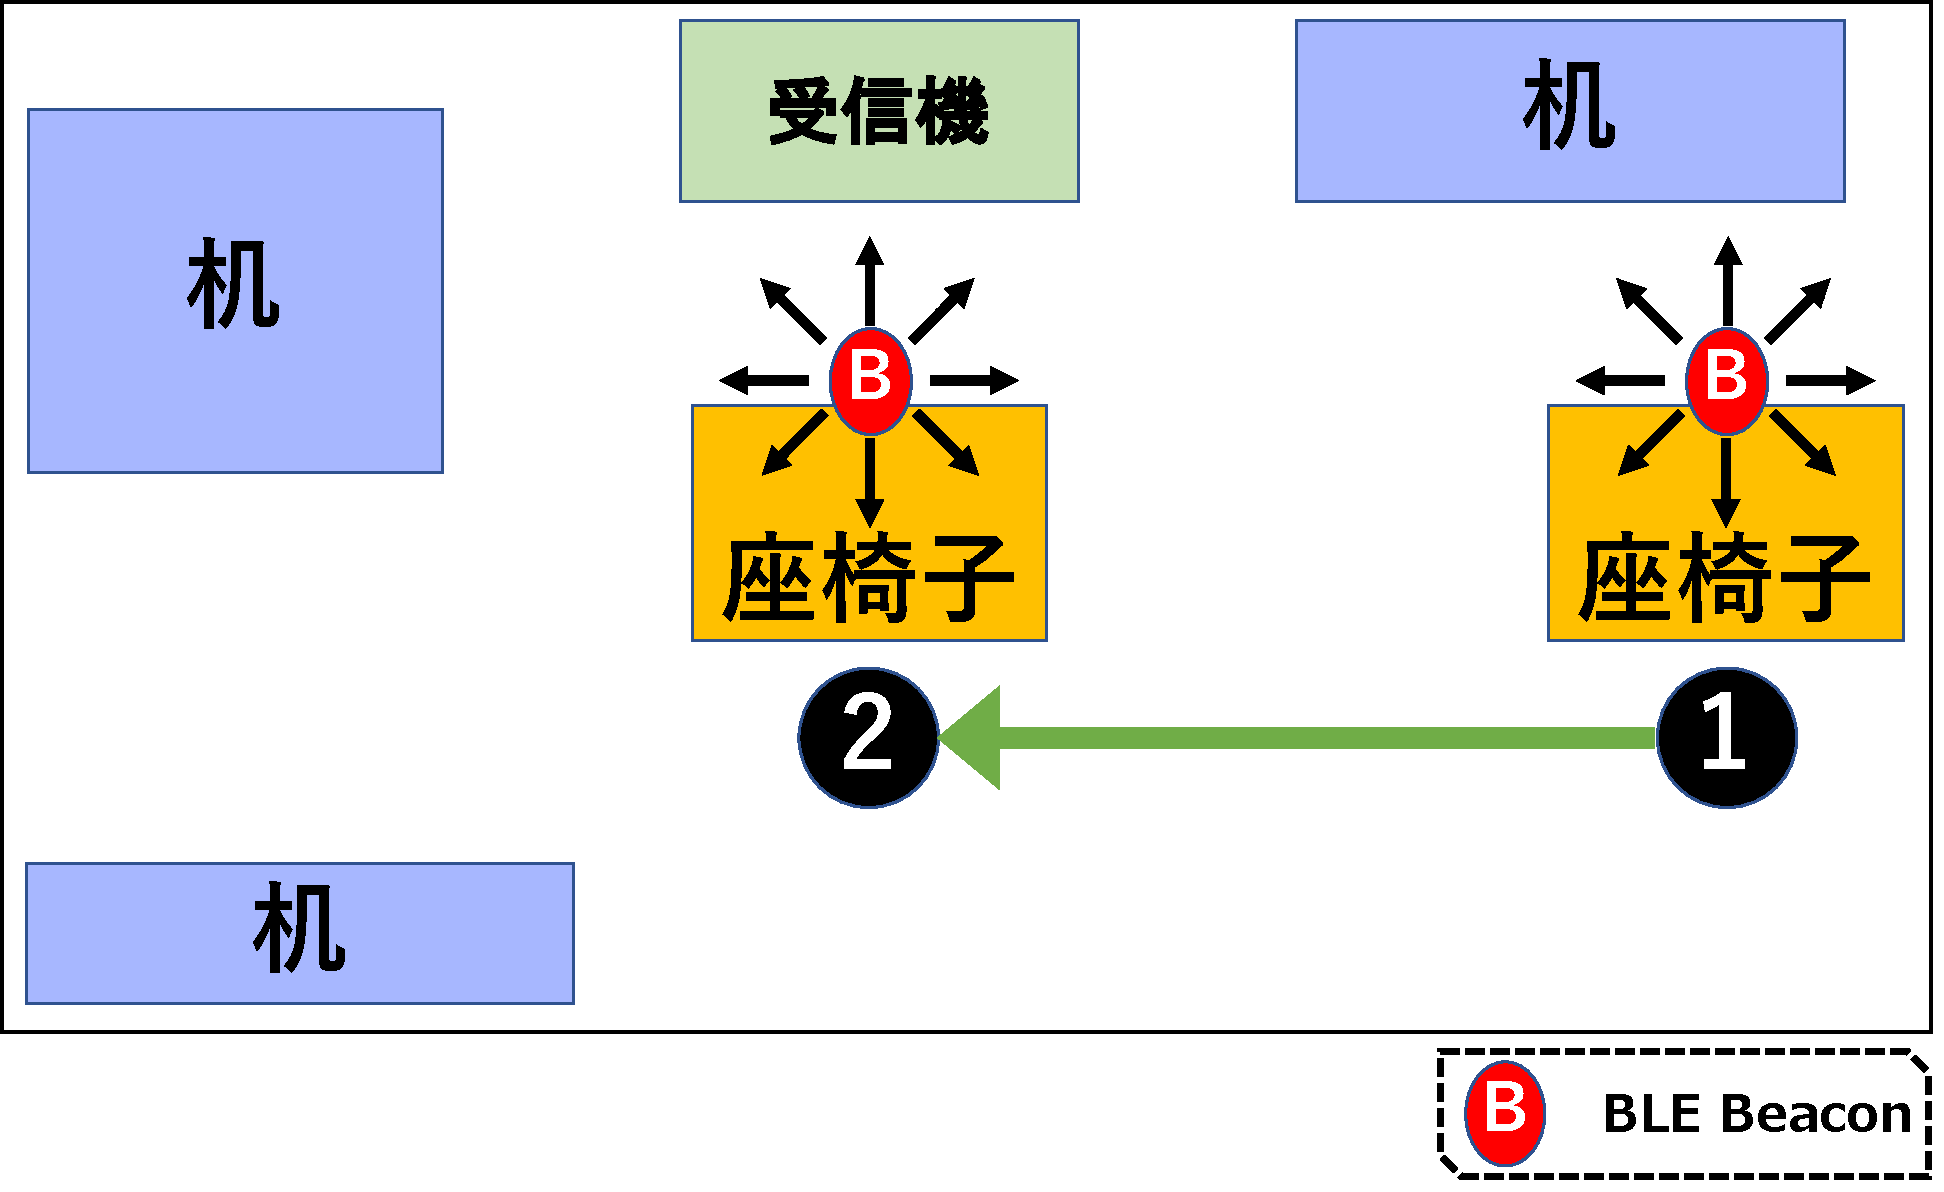
\includegraphics[width=10cm]{images/chapter3/zaisu_position.pdf}
    \caption{座椅子と受信機の位置関係図}
    \label{zaisu_position}
\end{figure}


\begin{figure}[tbh]
    \centering
    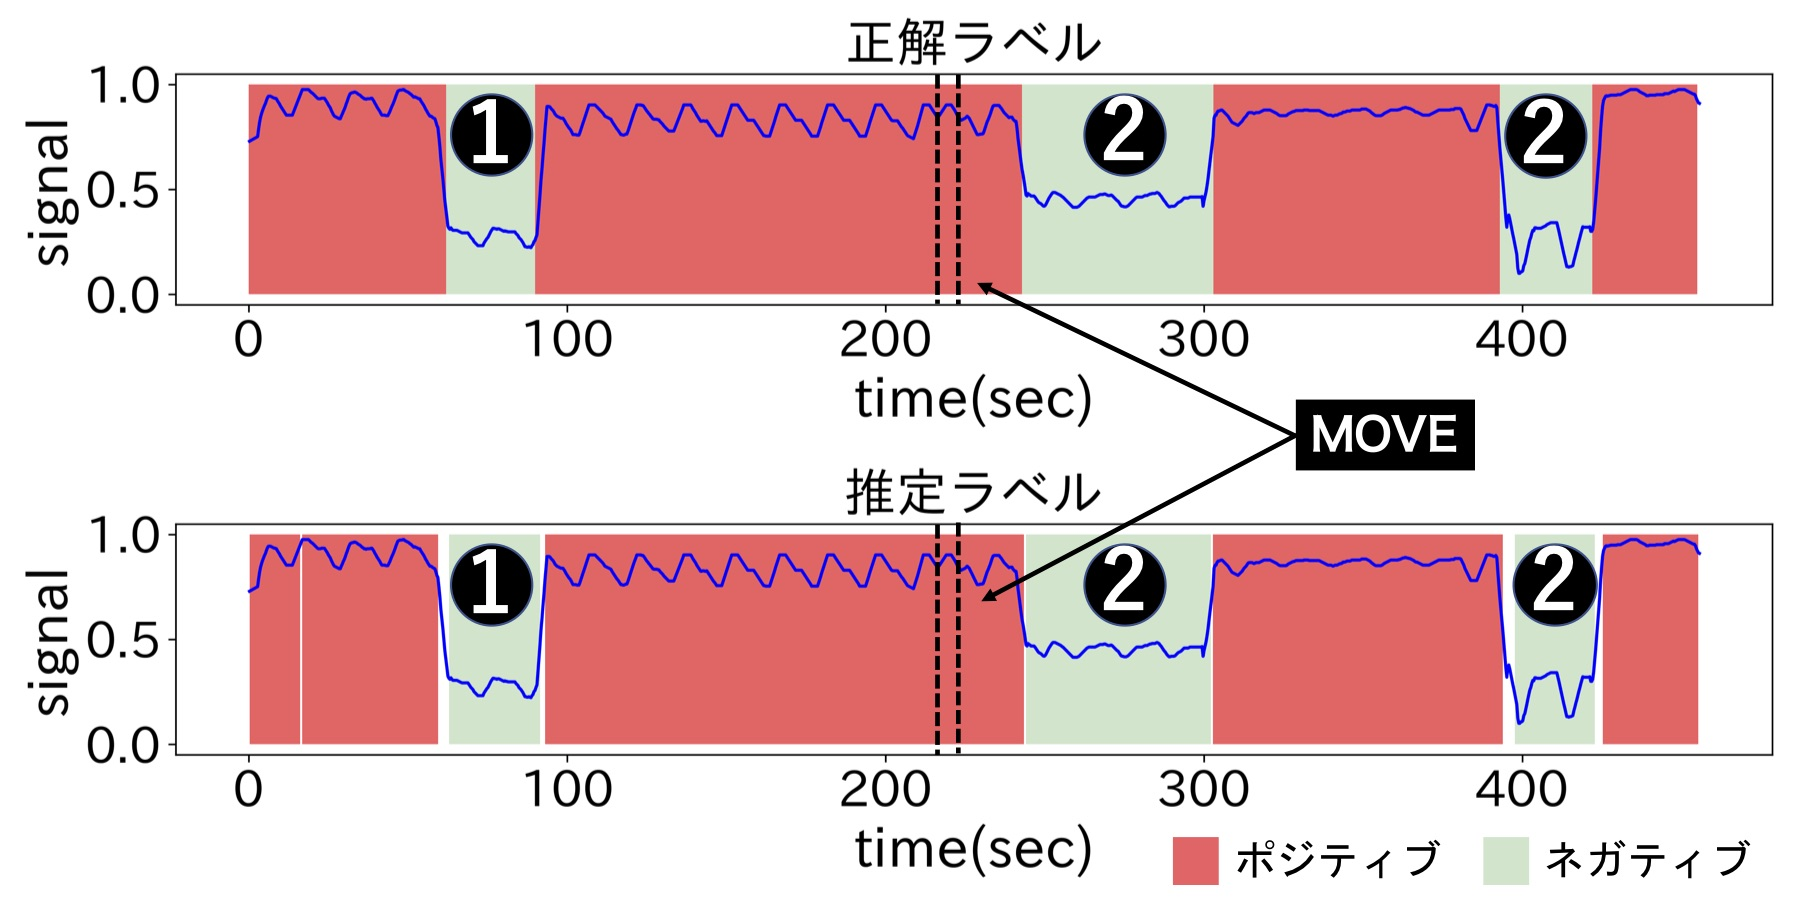
\includegraphics[width=14cm]{images/chapter3/zaisu_graph.jpg}
    \caption{座椅子の状態推定結果グラフ}
    \label{chair_graph}
\end{figure}


\begin{table}[tbh]
    \begin{center}
        \caption{座椅子への着席における状態推定精度}
        \label{chair_fig}
        \begin{tabular}{|c|c|c|c|} \hline
        試行回数 & 正答率 & 正解数 & 不正解数 \\ \hline
        1 & 100\% & 7 & 0 \\ \hline
        2 & 100\% & 7 & 0 \\ \hline
        3 & 100\% & 7 & 0 \\ \hline \hline
        回数でみた累計正解率 & \multicolumn{3}{c|}{100\%} \\ \hline \hline
        推定ラベルの正解割合 & \multicolumn{3}{c|}{98.9\%} \\ \hline

        \end{tabular}
    \end{center}
\end{table}


\section{考察}
評価実験の結果,冷蔵庫の開閉は99.2\%,金庫の開閉は93.8\%,座椅子の着座は98.9\%の精度で推定可能であり,提案手法の有効性を確認できた.
座椅子の状態変化では,受信電波強度が大きく変化したため,安定センシング区間が正解ラベルに近い状態で判定されており,冷蔵庫や金庫より高い推定精度であった.
人体は多く水分を含んでいるため電波を遮りやすく,人が座っていない時と座っている時の電波強度の変化が大きい.
それによりBLEビーコン特有の周期的な電波強度の変化に影響されず,正しく推定ができたと考えられる.

一方で,冷蔵庫と金庫の開閉では安定センシング区間の判定が上手くできていなかったため,誤推定された箇所があった.
これはBLEビーコン特有の周期的な電波強度の変化が安定センシング区間の判定に影響するため,少し大きめの閾値を取った結果,電波強度の変化がこの閾値を超えられなかったと考えられる.
そのため,状態が変化した後であっても前の状態が続いていると判定されてしまい,推定結果にも影響を及ぼした.
従って,推定精度を更に高めるには,安定センシング区間の判定に用いる閾値を見直す必要があるだろう.

%どんなものが出来て出来ないか
本稿の評価実験で扱ったモノの他に,状態変化により電波強度が大きく変化し提案手法が適用できるモノとして,椅子,お店のシャッター,金属製のキャビネットなどいくつかあったが,変化が現れず適用できないモノや状況もあった.
例えば木製のドアや引き出し,ギターケースなどの電波を減衰させにくい材質のモノでは状態変化しても電波強度の変化が少なく状態推定が難しい.
また,提案手法では指向性アダプタを取り付けて電波強度に大きな変化を出すようにしたが,電波が一方向にしか飛ばなくなる.
そのため,指向性アダプタが受信機の方を向いて状態変化が行われないと,電波強度の変化を捉えられないため状態推定を行うのは難しい.

また,本研究では状態がネガティブ・ポジティブの2値であるモノの状態推定を行ってきたが,状態が2値だけでないモノもある.
日常生活空間内にはゴミの累積や服の増減など,状態が推移していくモノもあるためそちらへの対応もする必要もあるだろう.

\thispagestyle{myheadings}
\addcontentsline{toc}{chapter}{\protect\numberline {} 参考文献}

\bibliography{reference} %hoge.bibから拡張子を外した名前
\bibliographystyle{junsrt} %参考文献出力スタイル

\appendix
\end{document}
